% This is part of Mes notes de mathématique
% Copyright (c) 2011-2014
%   Laurent Claessens
% See the file fdl-1.3.txt for copying conditions.

%+++++++++++++++++++++++++++++++++++++++++++++++++++++++++++++++++++++++++++++++++++++++++++++++++++++++++++++++++++++++++++
\section{Généralités}
%+++++++++++++++++++++++++++++++++++++++++++++++++++++++++++++++++++++++++++++++++++++++++++++++++++++++++++++++++++++++++++

\begin{definition}  \label{DefTMNooKXHUd}
    Un \defe{corps}{corps} est un anneau non nul dans lequel tout élément non nul est inversible.
\end{definition}

\begin{remark}
    Nous trouvons parfois le terme \defe{anneau à division}{anneau!à division}. Cela provient du fait que dans beaucoup de cas on considère uniquement des corps commutatifs; donc on voudrait une façon de parler d'un anneau dont tous les éléments non nuls sont inversibles. Dans ce cadre on dit :
    \begin{itemize}
        \item Un anneau à division est un anneau dont tous les éléments non nuls sont inversibles,
        \item Un corps est un anneau à division commutatif.
    \end{itemize}
    Pour prendre un exemple de cette différence, le théorème de Wedderburn \ref{ThoMncIWA} est énoncé ici sous les termes «Tout corps fini est commutatif». Sous-entendu : la commutativité ne fait pas partie de la définition d'un corps. Par contre dans \cite{KXjFWKA} il est énoncé sous les termes «Tout anneau à division fini est un corps». Chez lui, un corps est toujours commutatif et un anneau à division est ce que nous appelons ici un corps.
    
    Dans tous les cas, un corps dans lequel l'élément nul est inversible est appelé un mensonge, comme le prouve le lemme suivant.
\end{remark}

\begin{lemma}       \label{LemAnnCorpsnonInterdivzer}
    En tant que anneau, un corps est un anneau intègre : il n'a pas de diviseurs zéro. 
\end{lemma}
Dans un corps nous avons toujours la règle du produit nul.

\begin{proof}
    En effet si \( a\) est un diviseur de zéro, alors \( ax=0\) pour un certain \( x\neq 0\). Si \( a\) était inversible, nous aurions \( x=a^{-1}ax=0\), ce qui est impossible.
\end{proof}

\begin{definition}[Algèbre\cite{ZSyHmiy}]   \label{DefAEbnJqI}
    Si \( \eK\) est un corps commutatif\footnote{Définition \ref{DefTMNooKXHUd}}, une \( \eK\)-\defe{algèbre}{algèbre} \( A\) est un espace vectoriel muni d'une opération bilinéaire \( \times\colon A\times A\to A\), c'est à dire telle que pour tout \( x,y,z\in A\) et pour tout \( \alpha,\beta\in\eK\),
    \begin{enumerate}
        \item
            \( (x+y)\times z=x\times z+y\times z\)
        \item
            \( x\times (y+z)=x\times y+x\times z\)
        \item
            \( (\alpha x)\times (\beta y)=(\alpha\beta)(x\times y)\).
    \end{enumerate}
    Si \( A\) et \( B\) sont deux \( \eK\)-algèbres, une application \( f\colon A\to B\) est un \defe{morphisme}{morphisme!d'algèbres} entre \( A\) et \( B\) si pour tout \( x,y\in A\) et pour tout \( \alpha\in \eK\),
    \begin{enumerate}
        \item
            \( f(xy)=f(x)f(y)\)
        \item
            \( f(x+\alpha y)=f(x)+\alpha f(y)\)
    \end{enumerate}
    où nous avons noté \( xy\) pour \( x\times y\).
\end{definition}


Par le lemme \ref{LemCaractIntergernbrcartpre}, un anneau sans diviseur de zéro est de caractéristique zéro ou première. Le fait d'être intègre pour un anneau n'assure cependant pas le fait d'être un corps. Nous avons cependant ce résultat pour les anneaux finis.

\begin{proposition}     \label{PropanfinintimpCorp}
    Un anneau fini intègre est un corps.
\end{proposition}

\begin{proof}
    Soit \( A\) un tel anneau. Soit \( a\neq 0\). Les applications 
    \begin{subequations}
        \begin{align}
            l_a\colon x\to ax\\
            r_a\colon x\to xa
        \end{align}
    \end{subequations}
    sont injectives. En tant que applications injectives entre ensembles finis, elles sont surjectives. Il existe donc \( b\) et \( c\) tels que \( 1=ba=ac\). Il se fait que \( b\) et \( c\) sont égaux parce que
    \begin{equation}
        b=b(ac)=(ba)c=c.
    \end{equation}
    Par conséquent \( b\) est un inverse de \( a\).
\end{proof}

\begin{proposition}     \label{PropzhFgNJ}
    Soit \( n\in\eN^*\). Les conditions suivantes sont équivalentes :
    \begin{enumerate}
        \item
            \( n\) est premier.
        \item
            \( \eZ/n\eZ\) est un anneau intègre.
        \item
            \( \eZ/n\eZ\) est un corps.
    \end{enumerate}
\end{proposition}

\begin{proof}
    L'équivalence entre les deux premiers points est le contenu du corollaire \ref{CorZnInternprem}. Le fait que \( \eZ/n\eZ\) soit un corps lorsque \( \eZ/n\eZ\) est intègre est la proposition \ref{PropanfinintimpCorp}. Le fait que \( \eZ/n\eZ\) soit intègre lorsque \( \eZ/n\eZ\) est un corps est une propriété générale des corps : ce sont en particulier des anneaux intègres (lemme \ref{LemAnnCorpsnonInterdivzer}).
\end{proof}

\begin{proposition}     \label{AnnCorpsIdeal}
    Si \( A\) est un anneau, nous avons les équivalences
    \begin{enumerate}
        \item
            \( A\) est un corps.
        \item
            \( A\) est non nul et ses seuls idéaux à gauche sont \( \{ 0 \}\) et \( A\).
        \item
            \( A\) est non nul et ses seuls idéaux à droite sont \( \{ 0 \}\) et \( A\).
    \end{enumerate}
\end{proposition}

\begin{proposition}
    Soit \( A\), un anneau commutatif non nul et \( I\), un idéal dans \( A\). L'ensemble \( I\) est un idéal maximum de \( A\) si et seulement si \( A/I\) est un corps.
\end{proposition}

\begin{proof}
    Par la proposition \ref{AnnCorpsIdeal}, le fait pour \( A/I\) d'être un corps signifie qu'il n'a pas d'idéaux non triviaux. Si \( \phi\) est la projection canonique \( A\mapsto A/I\), nous savons que les idéaux de \( A/I\) sont les \( \phi(J)\) où \( J\) est un idéal de \( A\) contenant \( I\) (proposition \ref{PropIJJIdsousphi}). Si \( I\) est un idéal maximum de \( A\), un tel \( J\) n'existe pas. Inversement si \( A/I\) n'a pas d'autres idéaux que \( A/I\) et \( \phi(0)\), c'est que \( I\) est un idéal maximum.
\end{proof}

%---------------------------------------------------------------------------------------------------------------------------
\subsection{Corps des fractions}
%---------------------------------------------------------------------------------------------------------------------------

\begin{theorem}     \label{ThogbhWgo}
    Soit \( \eA\) un anneau commutatif intègre. Il existe un corps commutatif \( \eK\) et un morphisme injectif (d'anneaux) \( \epsilon\colon \eA\to \eK\) tels que pour tout \( \lambda\in\eK\), il existe \( (a,b)\in \eA\times \eA^*\) tels que
    \begin{equation}
        \lambda=\epsilon(a)\big( \epsilon(b) \big)^{-1}
    \end{equation}

    De plus si \( (\eK',\epsilon')\) est un autre couple qui vérifie la propriété, les corps \( \eK\) et \( \eK'\) sont isomorphes.
\end{theorem}
Le corps \( \eK\) associé à l'anneau \( \eA\) est le \defe{corps des fractions}{corps!des fractions}\index{fractions (corps)} de \( \eA\), et sera noté \( \Frac(\eA)\).\nomenclature[A]{\( \Frac(\eA)\)}{Le corps des fractions de l'anneau \( \eA\)}

Notons que l'application \( \eA\times \eA^*\to \eK\) donnée par \( (a,b)\mapsto \epsilon(a)\big( \epsilon(b) \big)^{-1}\) envoie \( (xa,xb)\) sur le même que \( (a,b)\).

L'ensemble \( \eQ\)\nomenclature[A]{\( \eQ\)}{corps des fractions sur \( \eZ\)} est le corps des fractions de \( \eZ\).

%---------------------------------------------------------------------------------------------------------------------------
\subsection{Corps premier}
%---------------------------------------------------------------------------------------------------------------------------
\label{subseccorpspremhBlYIv}

\begin{definition}
    Un corps est \defe{premier}{corps!premier}\index{premier!corps} si il est son seul sous corps. Le \defe{sous corps premier}{premier!sous corps} d'un corps est l'intersection de tous ses sous corps.
\end{definition}

\begin{lemma}
    Un corps premier est commutatif
\end{lemma}

\begin{proof}
    Le centre d'un corps est certainement un sous corps. Par conséquent un corps premier doit être contenu dans son propre centre, c'est à dire être commutatif.
\end{proof}

Soit \( p\) un nombre premier. Nous notons \( \eF_p=\eZ_p=\eZ/p\eZ\)\nomenclature[A]{\( \eF_p\)}{lorsque \( p\) est premier}. 

Nous verrons plus loin (section \ref{SecCorpsFinizkAcbS}) comment nous pouvons définir \( \eF_{p^n}\) lorsque \( p\) est premier, ainsi que l'unicité d'un tel corps.

Nous avons par exemple 
\begin{equation}
    \eF_2=\eZ/2\eZ=\{ 0,1 \}
\end{equation}
avec la loi \( 2=0\).

Notons que \( \eF_p\) est un corps possédant \( p\) éléments. L'ensemble \( \eF_p^*\) est un groupe d'ordre \( p-1\).

\begin{lemma}
    Les corps \( \eQ\) et \( \eF_p\) (avec \( p\) premier) sont premiers.
\end{lemma}

\begin{proof}
    Tout sous corps de \( \eQ\) doit contenir \( 1\), et par conséquent \( \eZ\). Devant également contenir tous les inverses, il contient \( \eQ\).

    Tout sous corps de \(\eF_p \) doit contenir \( 1\) et donc \( \eF_p\) en entier. Par ailleurs nous savons de la proposition \ref{PropzhFgNJ} que \( \eF_p\) est un corps lorsque \( p\) est premier.
\end{proof}

\begin{proposition}
    Soit \( \eK\) un corps de caractéristique \( p\) et \( \eP\) son sous corps premier. Si \( p=0\) alors \( \eP=\eQ\). Si \( p>0\), alors \( \eP=\eF_p\).
\end{proposition}

\begin{proof}
    Notons d'abord que la caractéristique d'un corps est toujours un nombre premier parce qu'un corps est en particulier un anneau intègre (proposition \ref{LemCaractIntergernbrcartpre}).

    Étant donné que \( 1\) est dans tout sous corps, nous devons avoir \( \eZ 1\subseteq \eP\). Si \( p=0\), alors \( \eZ 1\simeq \eZ\), et nous avons
    \begin{equation}
        \eZ 1_{\eA}\subset \eP\subset \eK.
    \end{equation}
    Pour chaque \( (n,m)\in \eZ 1_{\eA}\times (\eZ 1_{\eA})^*\) l'élément \( nm^{-1}\in \eK\) est dans \( \eP\) parce que \( \eP\) est un corps. Nous en déduisons que le corps des fractions de \( \eZ\) est contenu dans \( \eP\) par conséquent \( \eP=\eQ\) (théorème \ref{ThogbhWgo}). 

    Si par contre la caractéristique de \( \eK\) est \( p\neq 0\), nous avons \( \eZ 1_{\eA}\simeq\eZ/p\eZ=\eF_p\) par le lemme \ref{LemHmDaYH}. L'ensemble \( \eF_p\) étant un corps, c'est le corps premier de \( \eK\).
\end{proof}

\begin{proposition}     \label{PropqPPrgJ}
    Soit \( \eK\) un corps et \( \eP\) sont sous corps premier. Si \( \sigma\in\Aut(\eK)\) alors \( \sigma|_{\eP}=\id\), c'est à dire que
    \begin{equation}
        \sigma(x)=x
    \end{equation}
    pour tout \( x\in \eP\).
\end{proposition}

\begin{theorem}[Théorème de Gauss]  \label{ThoLLgIsig}
    Soient \( P,Q,R\in \eK[X]\) tels que \( P\) soit premier avec \( Q\) et divise \( QR\). Alors \( P\) divise \( R\).
\end{theorem}
\index{théorème!Gauss!polynômes}

\begin{proof}
    Étant donné que \( P\) est premier avec \( Q\), le théorème de Bézout\footnote{théorème \ref{ThoBezoutOuGmLB}.} nous donne \( U,V\in \eK[X]\) tels que \( PU+QV=1\). De plus il existe un polynôme \( S\) tel que \( PS=QR\). En multipliant l'identité de Bézout par \( R\), nous obtenons
    \begin{equation}
        R=PUR+QVR=PUR+VPS=P(UR+VS),
    \end{equation}
    ce qui signifie que \( P\) divise \( R\).
\end{proof}

Le lemme suivant est une généralisation du lemme de Gauss dans \( \eZ\) (lemme \ref{LemSdnZNX}).
\begin{lemma}[Lemme de Gauss\cite{fJhCTE}]       \label{LemEfdkZw}   \index{lemme!Gauss!polynômes}\index{Gauss!lemme!polynômes}
    Soient les polynômes unitaires \( P,Q\in \eQ[X]\). Si \( PQ\in\eZ[X]\), alors \( P\) et \( Q\) sont tous deux dans \( \eZ[X]\).
\end{lemma}

\begin{proof}
    Soit \( a>0\) le plus petit entier tel que \( aP\in\eZ[X]\) (c'est le PPCM des dénominateurs) et de la même façon \( b>0\) le plus petit entier tel que \( bQ\in \eZ[X]\). On pose \( P_1=aP\) et \( Q_1=bQ\).

    Si \( ab=1\), alors \( a=b=1\) et nous avons tout de suite \( P,Q\in \eZ[X]\). Nous supposons donc \( ab>1\) et nous considérons \( p\), un diviseur premier de \( ab\). Ensuite nous considérons la projection
    \begin{equation}
        \pi_p\colon \eZ[X]\to (\eZ/p\eZ)[X].
    \end{equation}
    Par définition \( abPQ=P_1Q_1\in \eZ[X]\); en prenant la projection,
    \begin{equation}
        \pi_p(P_1)\pi_p(Q_1)=\pi_p(P_1Q_1)=\pi_P(ab)\pi_p(PQ)=0
    \end{equation}
    parce que \( \pi_p(ab)=0\). Étant donné que \( (\eZ/p\eZ)[X]\) est intègre (exemple \ref{ExybCZyl}), nous avons soit \( \pi_p(P_1)=0\) soit \( \pi_p(Q_1)=0\). Supposons pour fixer les idées que \( \pi_p(P_1)=0\). Alors \( P_1=pP_2\) pour un certain \( P_2\in \eZ[X]\). Par ailleurs \( P\) est unitaire et \( P_1=aP\), donc le coefficient de plus haut degré de \( P_1\) est \( a\), et nous concluons que \( p\) divise \( a\).
    
    Mettons \( a=pa'\). Dans ce cas, \( pa'P=P_1=pP_2\), et donc \( a'P=P_2\in \eZ[X]\). Cela contredit la minimalité de \( a\).
\end{proof}

%---------------------------------------------------------------------------------------------------------------------------
\subsection{Petit théorème de Fermat}
%---------------------------------------------------------------------------------------------------------------------------

\begin{theorem}[Petit théorème de Fermat]       \label{ThoOPQOiO}   \index{théorème!petit de Fermat}\index{petit théorème de Fermat}
    Soit \( p\) un nombre premier. Si \( x\in \eF_p\) alors \( x^p=x\). Si \( x\in(\eF_p)^*\), alors \( x^{p-1}=1\).

    En particulier si \( x\in \eF_p^*\) alors \( x^{-1}=x^{p-2}\).
\end{theorem}

\begin{proof}
    Étant donné que \( \eF_p\) est un corps commutatif et que \( p\) est premier, la proposition \ref{Propqrrdem} nous indique que \( \sigma(x)=x^p\) est un automorphisme. La proposition \ref{PropqPPrgJ} nous indique alors que
    \begin{equation}
        a^p=a.
    \end{equation}
    Si \( a\) est inversible alors \( a^{p-1}=a^pa^{-1}=1\).
\end{proof}

\begin{remark}      \label{RemCoSnxh}
    Une autre façon d'énoncer le petit théorème de Fermat \ref{ThoOPQOiO} est que si \( p\) est premier et si \( a\) est premier avec \( a\), alors \( a^{p-1}\in[1]_p\). Le nombre \( a\) n'est pas premier avec \( p\) uniquement lorsque \( a\) est multiple de \( p\). Dans ce cas c'est \( a=0\) dans \( \eF_p\) et donc \( a^{p-1=0}\).
\end{remark}

\begin{example}
    Soit \( \eK=\eF_{29}^*\). Le nombre \( 29\) étant premier, \( \eK\) est un corps premier. C'est le corps des entier modulo \( 29\). Nous avons donc
    \begin{equation}
            -142=-113=-84=-55=-26=3=32=61=90=119.
    \end{equation}
    Le petit théorème de Fermat nous permet aussi de calculer des exposants et des inverses. Nous avons
    \begin{equation}
        x^{-a}=(x^a)^{27}=x^{27a}.
    \end{equation}
    Le nombre \( 27 a\) peut être grand par rapport à \( 29\). Étant donné que \( 1=x^{28}\) nous avons
    \begin{equation}
        x^{-a}=x^{27 a\mod 28}.
    \end{equation}
    Dans les exposants nous calculons modulo \( 28\).
\end{example}

%---------------------------------------------------------------------------------------------------------------------------
\subsection{Résultats chinois}
%---------------------------------------------------------------------------------------------------------------------------

Nous allons maintenant parler du système d'équations
\begin{subequations}
    \begin{numcases}{}
        x=a_1\mod p\\
        x=a_2\mod q
    \end{numcases}
\end{subequations}
avec \( a_1\), \( a_2\) donnés dans \( \eZ\) et \( p,q\) des entiers premiers entre eux. Le lemme chinois nous donne la liste des solutions ainsi qu'une manière de les construire. Le théorème chinois en sera une espèce de corollaire qui établira l'isomorphisme d'anneaux \( \eZ/pq\eZ\simeq \eZ/p\eZ\times \eZ/q\eZ\). Voir \href{http://www.les-mathematiques.net/b/a/d/node10.php}{les-mathematiques.net}.

\begin{lemma}[Lemme chinois \cite{CongrDuchSyl}]        \label{LemCtUeGA}
    Soient \( n_1,n_2\) deux entiers premiers entre eux. Soient \( a_1,a_2\in \eZ\). Les solutions du système
    \begin{subequations}        \label{SysVwvLKv}
        \begin{numcases}{}
            x=a_1\mod n_1\\
            x=a_2\mod n_2
        \end{numcases}
    \end{subequations}
    pour \( x\in \eZ/n_1n_2\eZ\) sont données de la façon suivante. Soient \( u_1,u_2\) deux entiers qui satisfont la relation de Bézout\footnote{voir le théorème \ref{ThoBuNjam}}
    \begin{equation}        \label{EqWcucUG}
        u_1n_1+u_2n_2=1,
    \end{equation}
    et 
    \begin{equation}        \label{EqHGchlQ}
        a=\big( a_1u_2n_2+a_2 u_1n_1 \big)\mod(n_1).
    \end{equation}
    Alors \( x=a\mod(n_1n_2)\).
\end{lemma}

\begin{proof}
    Vérifions que le \( x\) donné par \(x=a\mod(n_1n_2)\) est bien une solution. D'abord
    \begin{subequations}
        \begin{align}
            a\mod n_2&=a_1u_2n_2\mod n_1\\
            &=a_1(1-u_1n_1)\mod n_1\\
            &=a_1\mod n_1
        \end{align}
    \end{subequations}
    où nous avons utilisé l'identité de Bézout \eqref{EqWcucUG}. La vérification de \( a\mod n_2=a_2\mod n_2\) est la même.

    Soit maintenant \( x\in \eZ/n_1n_2\eZ\) une solution du système \eqref{SysVwvLKv} et \( a\) donné par la formule \eqref{EqHGchlQ}. Alors
    \begin{subequations}
        \begin{align}
            (x-a)\mod n_1&=\Big( a_1-(a_1n_2u_2+a_2u_1n_1) \Big)\mod n_1\\
            &=a_1-a_1u_2n_2\mod n_1\\
            &=0,
        \end{align}
    \end{subequations}
    donc \( (x-a)\mod n_1=0\), ce qui signifie que \( x-a\) est divisible par \( n_1\). De la même façon, \( (x-a)\mod n_2=0\) et \( x-a\) est divisible par \( n_2\). Nous savons maintenant que \( x-a\) est divisible par \( n_1\) et \( n_2\). Étant donné que \( n_1\) et \( n_2\) sont premiers entre eux, nous en déduisons que \( x-a\) est divisible par \( n_1n_2\), ou encore que \( x=a\mod n_1n_2\).
\end{proof}

\begin{theorem}[Théorème chinois]
    Soient \( p,q\) deux naturels premiers entre eux. Si \( p,q\geq 2\) alors l'application
    \begin{equation}
        \begin{aligned}
            \phi\colon \eZ/pq\eZ&\to \eZ/p\eZ\times \eZ/q\eZ \\
            [x]_{pq}&\mapsto \big( [x]_p,[x]_q \big) 
        \end{aligned}
    \end{equation}
    est un isomorphisme d'anneaux.
\end{theorem}

\begin{proof}
    Nous devons prouver que l'application \( \phi\) respecte la somme, le produit et qu'elle est bijective. En ce qui concerne la somme,
    \begin{subequations}
        \begin{align}
            \phi([q]_{pq}+[y]_{pq})&=            \phi\big( (x+y)\mod pq \big)\\
            &=\big( [x+y]_{p},[x+y]_q \big)\\
            &=\big( [x]_p+[y]_p,[x]_q+[y]_q \big)\\
            &=\big( [x]_p,[x]_q \big)+\big( [y]_p,[y]_q \big)\\
            &=\phi(x)+\phi(y).
        \end{align}
    \end{subequations}
    En ce qui concerne le produit, c'est le même jeu : nous obtenons
    \begin{equation}
        \phi\big( [xy]_{pq} \big)=\phi([x]_{pq}])\phi([y]_{pq})
    \end{equation}
    en utilisant le fait que \( [xy]_{p}=[x]_p[y]_p\).

    Montrons maintenant que \( \phi\) est surjective. Soient \( y_1,y_2\in \eZ\) et \( x\in \eZ\). Demander
    \begin{equation}
        \phi([x]_{pq})=\big( [y_1]_p,[y_2]_q \big)
    \end{equation}
    revient à demander que \( [x]_p=[y_1]_p\) et \( [x]_q=[y_2]_q\), c'est à dire que \( x\) résolve le système
    \begin{subequations}
        \begin{numcases}{}
            x=y_1\mod p\\
            x=y_2\mod q.
        \end{numcases}
    \end{subequations}
    Le lemme chinois \ref{LemCtUeGA} nous assure qu'une solution existe.

    En ce qui concerne l'injectivité, nous supposons que \( x\) et \( y\) soient deux entiers tels que
    \begin{equation}
        \phi([x]_{pq})=\phi([y]_{pq}).
    \end{equation}
    Nous en déduisons le système
    \begin{subequations}
        \begin{numcases}{}
            x\mod p=y\mod p\\
            x\mod q=y\mod q
        \end{numcases}
    \end{subequations}
    c'est à dire qu'il existe des entiers \( k\) et \( l\) tels que \( x=y+kp\) et \( x=y+lq\) ou encore tels que
    \begin{equation}
        kp+lq=0.
    \end{equation}
    Étant donné que \( p\) et \( q\) sont premiers entre eux, la seule possibilité est \( k=l=0\), c'est à dire \( x=y\).
\end{proof}

\begin{theorem}[Théorème chinois]\index{théorème!chinois}
    Soit \( A\) un anneau commutatif, \( n\geq 2\), des éléments \( x_1,\ldots,x_n\) dans \( A\) et des idéaux \( I_1,\ldots,I_n\) tels que \( I_i+I_j=A\) pour tout \( i\neq j\).

    Alors il existe un \( x\in A\) tel que \( x-x_i\in I_i\) pour tout \( 1\leq i\leq n\).
\end{theorem}

\begin{proof}
    Pour \( i\in\{ 1,\ldots,n \}\) nous notons \( J_i\) le produit \( J_i=\prod_{k\neq i}I_k\). Étant donné que chaque \( I_i\) est un idéal, nous avons \( I_k\in J_i\) lorsque \( i\neq k\).

    Soit \( i\) fixé, et considérons \( j\neq i\). Nous pouvons trouver \( a_j\in I_i\) et \( b_j\in I_j\) tel que \( a_j+b_j=1\). Nous avons alors
    \begin{equation}
        1=\prod_{j\neq i}(a_j+b_j).
    \end{equation}
    Par ailleurs \( I_i+J_i=A\) parce que \( J_i\) contient \( I_k\) avec \( k\neq i\) et \( I_i+I_k=A\). Nous pouvons donc prendre \( \alpha_i\in I_i\) et \( \beta_i\in J_i\) tels que
    \begin{equation}
        \prod_{j\neq i}(a_j+b_j)=\alpha_i+\beta_i.
    \end{equation}
    Nous considérons alors l'élément \( x=\beta_1x_1+\ldots+\beta_nx_n\) et nous avons
    \begin{subequations}
        \begin{align}
            x-x_1&=(\beta_1-1)x_1+\beta_2x_2+\ldots+\beta_nx_n\\
            &=-\alpha_1x_1+\beta_2x_2+\ldots+\beta_nx_n
        \end{align}
    \end{subequations}
    Mais \( \alpha_1\in I_1\) et tous les autres termes sont dans les \( J_i\) avec \( i\neq 1\). Par conséquent le tout est dans \( I_1\). Ici nous utilisons par exemple le fait que \( \beta_2\in J_2\subset I_1\) parce que les éléments de \( J_2\) sont des produits d'éléments dont un facteur est dans \( I_1\).
\end{proof}

\begin{remark}
    Ce théorème chinois est bien une généralisation du lemme chinois \ref{LemCtUeGA}. En effet, l'élément \( x\) dont il est question est solution du problème \( x=x_i\mod I_i\). L'hypothèse \( I_i+I_j=A\) n'est pas nouvelle non plus étant donné que si \( p\) et \( q\) sont des entiers premiers entre eux nous avons \( p\eZ+q\eZ=\eZ\) par le corollaire \ref{CorgEMtLj}.
\end{remark}

%---------------------------------------------------------------------------------------------------------------------------
\subsection{Chiffrage RSA}
%---------------------------------------------------------------------------------------------------------------------------
\label{subSecEVaFYi}
\index{groupe!fini}
\index{groupe!permutation}
\index{groupe!partie génératrice}
\index{anneau!\( \eZ/n\eZ\)}
\index{nombre!premier}

Ce passage sur RSA provient en bonne partie de la \wikipedia{fr}{Rivest_Shamir_Adleman}{la page Wikipédia}.

Alice veut envoyer un message à Bob. L'idée est que Bob va donner à Alice une clef publique qui va permettre de chiffrer le message tandis que Bob va garder pour lui une clef privée qui permet de déchiffrer.

%///////////////////////////////////////////////////////////////////////////////////////////////////////////////////////////
\subsubsection{Mise en place par Bob}
%///////////////////////////////////////////////////////////////////////////////////////////////////////////////////////////

Bob se crée une paire de clef publique, clef privée de la façon suivante.
\begin{enumerate}
    \item
        Bob choisit deux nombres premiers distincts \( p,q\).
    \item
        Il calcule \( n=pq\) .
    \item
        Par le corollaire \ref{CorlvTmsf}, l'indicatrice d'Euler \( \varphi(n)=(p-1)(q-1)\) est facile à calculer pour Bob.
    \item
        Bob choisit \( e\in \eN\) premier avec \( \varphi(n)\), puis \( d\) tel que \( ed\in[1]_{\varphi(n)}\).
\end{enumerate}
Maintenant la paire est : clef publique \( (n,e)\) et clef privée \( (n,d)\)\footnote{Le fait que \( e\) soit public et \( d\) soit privé est une convention. \( e\) comme  \emph{encryption} et \( d\) comme \emph{decryption}.}.

Bob envoie la paire \( (n,e)\) à Alice. 

\begin{remark}
    Ici nous ne supposons pas que la communication soit sure. Une tierce personne peut intercepter le message. D'ailleurs en principe les gens publient leurs clef publique sur leurs sites, voire sur des sites dédiés. Le problème de l'identification reste à résoudre \wikipedia{en}{Key_signing_party}{à l'ancienne}.
\end{remark}

%///////////////////////////////////////////////////////////////////////////////////////////////////////////////////////////
\subsubsection{Chiffrement}
%///////////////////////////////////////////////////////////////////////////////////////////////////////////////////////////

Nous chiffrons en utilisant la clef publique \( (n,e)\). D'abord Alice se débrouille pour transformer son message en un nombre plus petit que \( n\). Soit \( M\) ce message. Alice code \( M\) en
\begin{equation}
    C=M^e\mod n.
\end{equation}
Tout le truc est que nous allons voir que l'application \( x\mapsto x^e\) est une bijection de \( \eF_n\) et que l'inverse est facile à calculer par Bob et difficile pour les autres. Alice envoie \( C\) à Bob. Encore une fois, nous ne supposons pas que cette communication soit privée. Le nombre \( C\) peut être intercepté.

%///////////////////////////////////////////////////////////////////////////////////////////////////////////////////////////
\subsubsection{Déchiffrage}
%///////////////////////////////////////////////////////////////////////////////////////////////////////////////////////////

Nous allons montrer que \( M=C^d\mod n\), et donc que Bob, connaissant \( (n,d)\), peut déchiffrer. D'abord
\begin{equation}
    C^d=(M^e)^d=M^{ed},
\end{equation}
mais nous savons qu'il existe \( k\) tel que
\begin{equation}
    ed=1+k\varphi(n)=1+k(p-1)(q-1).
\end{equation}
L'étape astucieuse est de remarquer que
\begin{equation}    \label{EqreeHgn}
    M^{1+k(p-1)(q-1)}\in [M]_p\cap[M]_q.
\end{equation}
Pour montrer cela nous utilisons le petit théorème de Fermat \ref{ThoOPQOiO} et la remarque \ref{RemCoSnxh}.
\begin{itemize}
    \item Si \( M\) est premier avec \( p\), alors \( M^{p-1}\in[1]_p\).
    \item Si \( M\) n'est pas premier avec \( p\), alors \( M\) est multiple de \( p\) et on sait que \( M^{p-1}\in[0]_p=[M]_p\).
\end{itemize}
Dans les deux cas nous avons \eqref{EqreeHgn}. Le nombre \( M^{1+k\varphi(n)}-M\) est donc à la fois multiple de \( p\) et de \( q\).

Le lemme chinois \ref{LemCtUeGA} nous dit immédiatement\footnote{C'est ici qu'il est important que \( p\) ne soit pas égal à \( q\). Si \( p=q\), alors le lemme chinois ne fonctionne pas.} qu'alors
\begin{equation}
    M^{1+k\varphi(n)}-M
\end{equation}
est un multiple de \( pq=n\), c'est à dire que
\begin{equation}
    C^d=M^{ed}\in [M]_n.
\end{equation}

Si on ne croit pas au lemme chinois, on peut utiliser le lemme de Gauss. Posons
\begin{equation}
    M^{1+k\varphi(n)}-M=ap=bq.
\end{equation}
Dans ce cas \( p\) divise \( bq\), mais \( q\) est premier avec \( p\), donc le lemme de Gauss \ref{LemSdnZNX} nous enseigne\footnote{Ici aussi, si \( p=q\), ça ne marche pas.} que \( p\) divise \( b\).

%///////////////////////////////////////////////////////////////////////////////////////////////////////////////////////////
\subsubsection{Une imprudence à ne pas commettre}
%///////////////////////////////////////////////////////////////////////////////////////////////////////////////////////////

Nous avons pris deux cas selon que \( M\) soit ou non premier avec \( p\). Une question qui arrive est la suivante : est-ce que c'est une bonne idée d'envoyer un message qui ne soit pas premier avec \( p\) ?

Si nous savons que \( M\) n'est pas premier avec \( p\), alors nous avons \( M^e=l^ep^e\) et \( n=pq\) qui sont publics. Donc un calcul de PGCD permettrait de trouver \( p\).

Il faut cependant savoir que 
\begin{itemize}
    \item La probabilité que ça arrive est infime : vu que \( M\) est entre \( 0\) et \( n=pq\), les multiples de \( p\) possibles sont \( p,2p,\cdots pq\). Il y a dont une chance sur \( p\) que cela arrive. Typiquement avec des \( p\) de l'ordre de \( 10^{120}\), on peut utiliser RSA chaque milliseconde sur chaque atome de l'univers depuis le début des temps que ça ne se serait presque certainement pas encore produit.
    \item
        De toutes façons Alice ne sait pas vérifier si son message est premier avec \( p\) parce qu'elle ne connaît pas \( p\).
    \item 
        En conclusion la partie de la preuve qui montre que \( M^{1+\varphi(n)}\in [M]_p\cap[M]_q\) dans le cas \( M\) non premier avec \( p\) est, à toutes fins pratiques, inutile parce que ce cas de figure ne se présentera jamais dans toutes l'histoire de l'univers, même pas avec une civilisation intelligente autour de chaque étoile.
\end{itemize}

%///////////////////////////////////////////////////////////////////////////////////////////////////////////////////////////
\subsubsection{Problèmes calculatoires}
%///////////////////////////////////////////////////////////////////////////////////////////////////////////////////////////

Pour implémenter RSA, il faut pouvoir faire (au moins) trois choses :
\begin{enumerate}
    \item
        Trouver de grands nombres premiers.
    \item
        Trouver des couples de Bézout.
    \item
        Calculer \( M^e\) lorsque \( e\) est très grand.
\end{enumerate}
En ce qui concerne le problème de trouver des nombres premiers, c'est compliqué, mais il faut savoir qu'il y en a plein. À \( 120\) chiffres, il y a environ autant de nombres premiers que d'atomes dans \( 10^{20}\) fois l'univers connu. Cela rend impossible toute tentative de factoriser un grand nombre en essayant toutes les possibilités. Même pas en science-fiction\footnote{Cela donne une idée des connaissances en math des klingons, dont le docteur Spock parvient à craquer le code mentalement en deux heures.}.

Trouver des nombres \( u\) et \( v\) tels que \( Au+Bv=\pgcd(A,B)\) est un problème expliqué en \ref{subSecIpmnhO}.

En ce qui concerne le calcul de \( M^e\) lorsque \( e\) est grand, il n'est évidemment pas pensable de faire \( M\cdot M\cdot\ldots M\) avec \( e\) facteurs. Un truc pour calculer en moins d'étapes est l'\defe{exponentiation rapide}{exponentielle!rapide}. Si \( e=2k\) est pair, nous calculons
\begin{equation}
    M^e=(M^k)^2;
\end{equation}
si \( e=2k+1\) alors nous calculons
\begin{equation}
    M^e=M(M^k)^2.
\end{equation}
Le calcul prend alors seulement environ \(  \log_2(e)  \) étapes. Pour donner une idée,
\begin{equation}
    \log_2(10^{120})\simeq 400.
\end{equation}
Très raisonnable, mais un ordinateur reste indispensable.

%///////////////////////////////////////////////////////////////////////////////////////////////////////////////////////////
\subsubsection{La solidité de RSA}
%///////////////////////////////////////////////////////////////////////////////////////////////////////////////////////////

La solidité de la méthode repose sur deux conjectures (non démontrées !!) :
\begin{itemize}
    \item Pour déchiffrer il \emph{faut} connaitre \( p\) et \( q\). 
    \item La difficulté de trouver \( p\) et \( q\) en partant de \( n=pq\) est exponentielle en \( n\).
\end{itemize}
Dans la méthode de déchiffrage proposée ici, \( p\) et \( q\) sont utilisés pour calculer \( d\) qui est solution de \( ed=[1]_{\varphi(n)}\). La seule formule connue pour calculer \( \varphi(n)\) est \( \varphi(n)=(p-1)(q-1)\). Si on trouve plus simple, alors RSA peut être craqué.

%///////////////////////////////////////////////////////////////////////////////////////////////////////////////////////////
\subsubsection{Note non mathématique pour doucher l'enthousiasme}
%///////////////////////////////////////////////////////////////////////////////////////////////////////////////////////////

Il est \href{https://www.torproject.org/about/torusers.html.en#activists}{souvent dit} que différents systèmes de chiffrement peuvent aider à avoir des discussions «discrètes» dans les régimes totalitaires. La technologie au service de la démocratie, voila qui enthousiasme la jeunesse. La réalité est qu'il est souvent possible de craquer un système de chiffrement arbitrairement complexe, même sans connaitre le petit théorème de Fermat \ldots

\begin{center}
        \ifpdf
            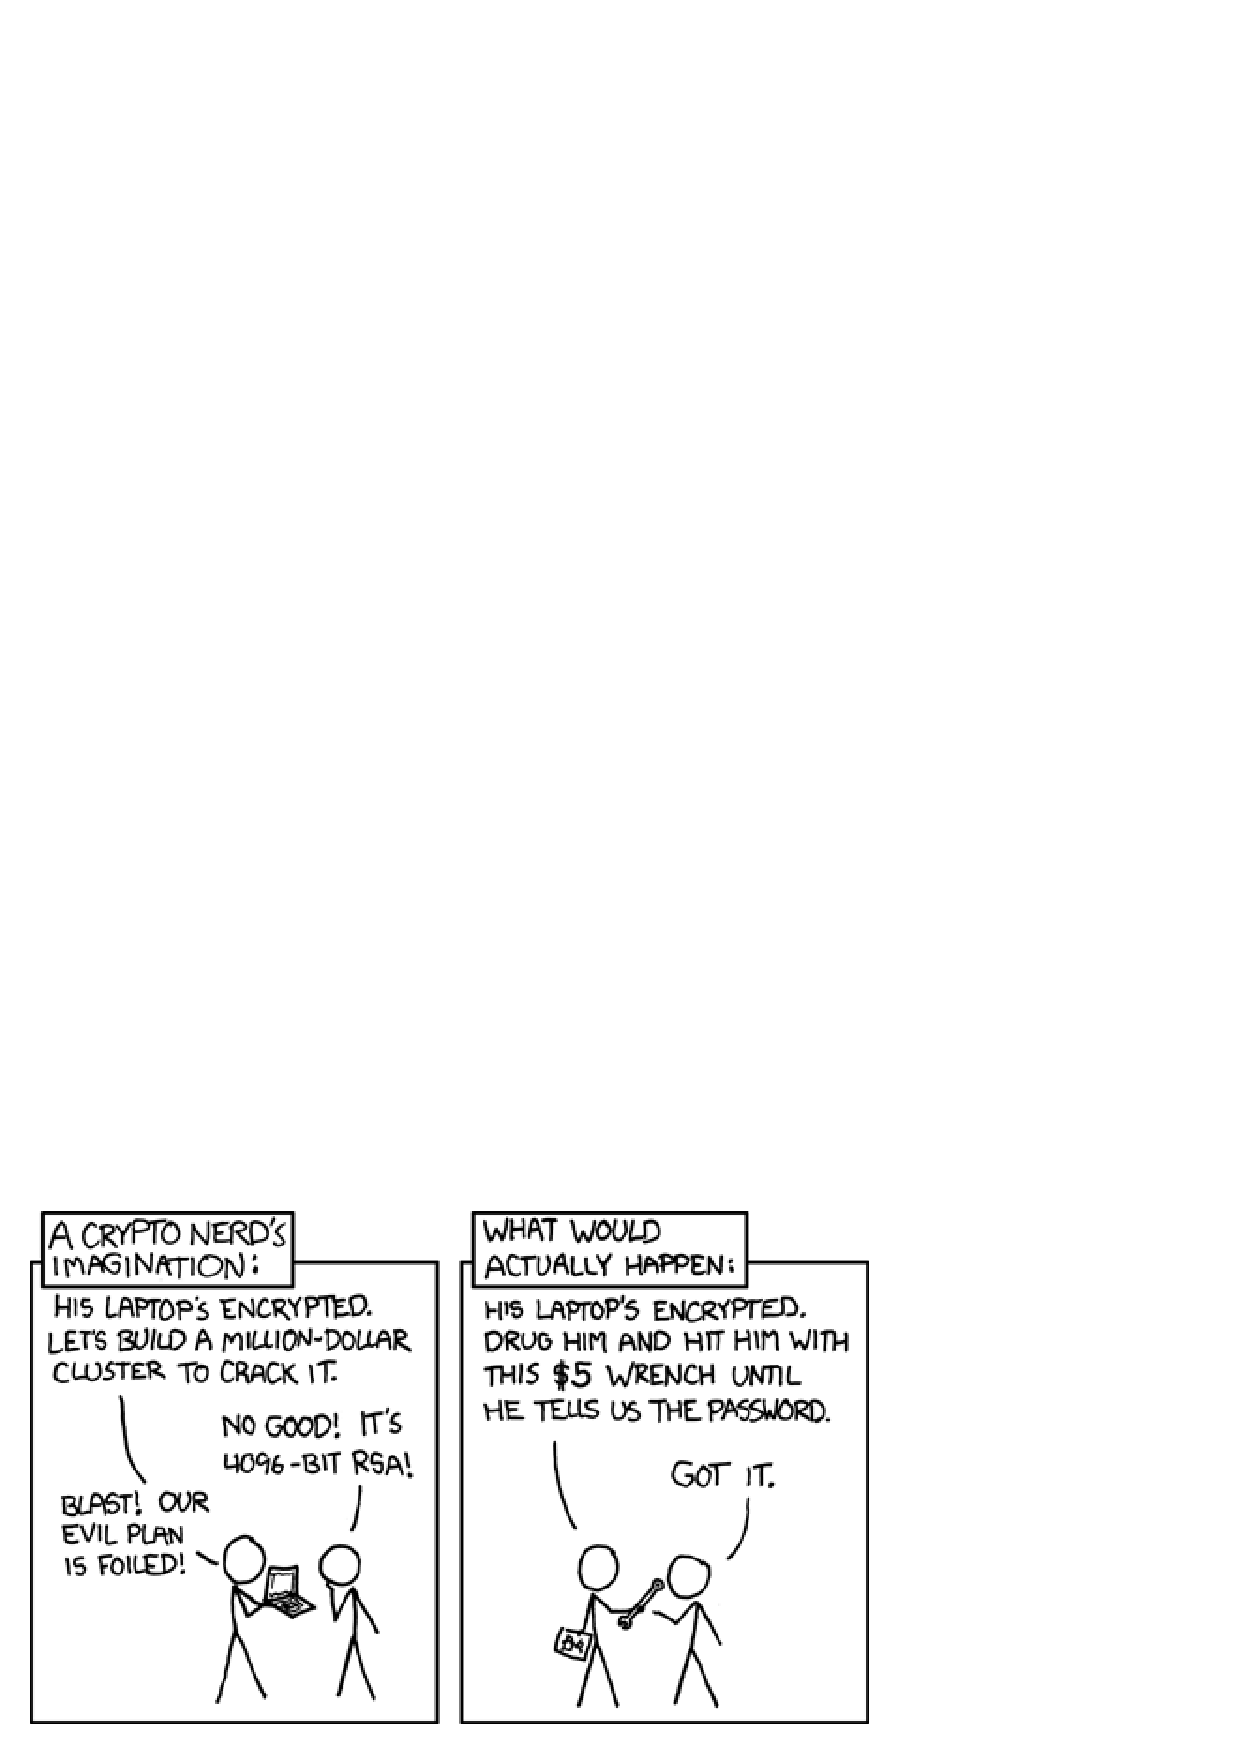
\includegraphics[width=10cm]{security.png}
        \else
            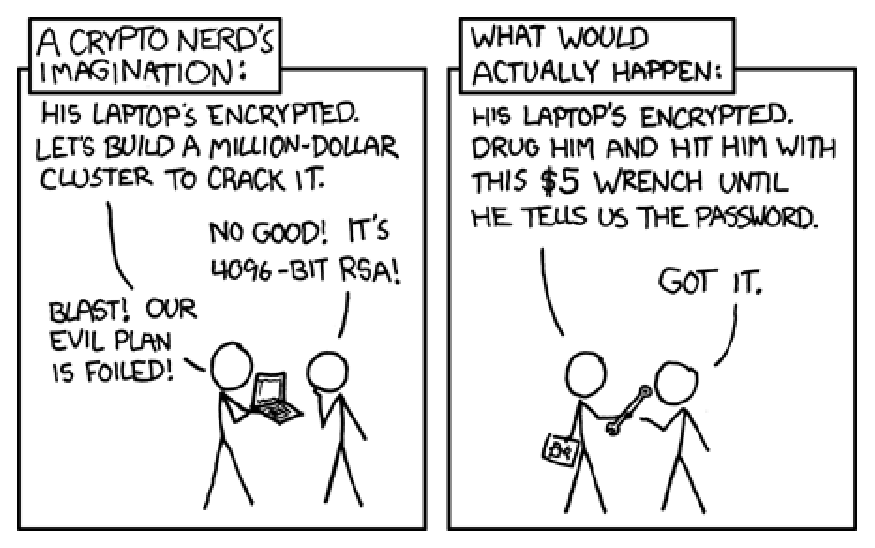
\includegraphics[width=10cm]{security.eps}
        \fi

        \url{http://xkcd.com/538/}. Ce dessin est publié sous licence \href{http://creativecommons.org/licenses/by-nc/2.5/}{ Creative Commons Attribution-NonCommercial 2.5 License}.
\end{center}

\noindent \ldots tout dépends du contexte.

%---------------------------------------------------------------------------------------------------------------------------
\subsection{Anneaux principaux et polynômes}
%---------------------------------------------------------------------------------------------------------------------------

Nous supposons que \( \eK\) est une corps commutatif, et nous étudions l'anneau \( \eK[X]\). Étant donné que \( \eK\) est commutatif pour tout polynôme que l'idéal engendré par \( P\) est \( (P)=\eK[X]P\), voir la notation \eqref{EqDefxMkDtW}.

\begin{remark}
    Un polynôme est irréductible dans \( \eK[X]\) au sens de la définition \ref{DeirredBDhQfA} si et seulement si il est irréductible au sens de la définition \ref{DefIrredfIqydS} parce que seules les constantes (non nulles) sont inversibles dans \( \eK[X]\).
\end{remark}

\begin{corollary}       \label{CorsLGiEN}
    Si \( \eK\) est un corps et si \( P\) est un polynôme irréductible de degré \( n\), alors l'ensemble \( \eL=\eK[X]/(P)\) est un corps. De plus \( \eL\) est un espace vectoriel de dimension \( n\).
\end{corollary}

\begin{proof}
    En effet \( \eK[X]\) est un anneau principal par le théorème \ref{ThoCCHkoU}, par conséquent la proposition \ref{PropoTMMXCx} déduit que \( \eK[X]/(P)\) est un corps.

    Une base de \( \eL\) est donnée par les projections de \( 1,X,X^2,\ldots, X^n\).
\end{proof}

%+++++++++++++++++++++++++++++++++++++++++++++++++++++++++++++++++++++++++++++++++++++++++++++++++++++++++++++++++++++++++++
\section{Extension de corps}
%+++++++++++++++++++++++++++++++++++++++++++++++++++++++++++++++++++++++++++++++++++++++++++++++++++++++++++++++++++++++++++

\begin{lemma}       \label{LemobATFP}
    Soit \( \eL\) un corps fini et \( \eK\) un sous corps de \( \eK\). Alors il existe \( s\in \eN\) tel que
    \begin{equation}        \label{EqUgqlJQ}
        \Card(\eK)=\Card(\eL)^s.
    \end{equation}
\end{lemma}

\begin{proof}
    Le corps \( \eL\) est un \( \eK\)-espace vectoriel de dimension finie. Si \( s\) est la dimension alors nous avons la formule \eqref{EqUgqlJQ} parce que chaque élément de \( \eL\) est un \( s\)-uple d'éléments de \( \eK\).
\end{proof}

\begin{definition}
    Soit \( \eK\) un corps commutatif. Une \defe{extension}{extension!de corps} de \( \eK\) est un corps \( \eL\) muni d'un morphisme \( i\colon \eK\to \eL\). Nous identifions le plus souvent \( \eK\) avec \( i(\eK)\subset \eL\).

    Une extension est \defe{algébrique}{extension!algébrique}\index{algébrique!extension} de \( \eK\) est une extension dont tous les éléments sont racines de polynômes dans \( \eK[X]\).
\end{definition}
Notons que \( \eR\) n'est pas une extension algébrique de \( \eQ\). En effet il existe seulement une infinité \emph{dénombrable} de polynômes dans \( \eQ[X]\) et donc une infinité dénombrable de racines de tels polynômes. Toute extension algébrique de \( \eQ\) est donc dénombrable.

%---------------------------------------------------------------------------------------------------------------------------
\subsection{Polynôme minimal}
%---------------------------------------------------------------------------------------------------------------------------

\begin{definition}[Polynôme minimal]    \label{DefCVMooFGSAgL}
    Soit \( \eL\) une extension de \( \eK\) et \( a\in \eL\). Nous considérons l'idéal
    \begin{equation}
        I_a=\{ P\in \eK[X]\tq P(a)=0 \}.
    \end{equation}
    Étant donné que \( \eK[X]\) est principal, cet idéal est principal et donc accepte un générateur unitaire. Nous nommons ce dernier \defe{polynôme minimal}{polynôme!minimal!d'un élément d'une extension} de \( a\) sur \( \eK\).
\end{definition}

\begin{example}
    Le polynôme minimal dépends du corps sur lequel on le considère. Par exemple le nombre imaginaire pur \( i\) accepte \( X-i\) comme polynôme minimal sur \( \eC\) et \( X^2+1\) sur \( \eQ[X]\).
\end{example}

\begin{proposition}[\cite{MonCerveau}]  \label{PropRARooKavaIT}
    Soit \( \eL\) un extension de \( \eK\) et \( a\in \eL\) dont le polynôme minimal sur \( \eK\) est \( \mu_a\in\eK[X]\). Alors
    \begin{enumerate}
        \item   \label{ItemDOQooYpLvXri}
            le polynôme \( \mu_a\) est irréductible\footnote{Définition \ref{DefIrredfIqydS}.} sur \( \eK\);
        \item
            si \( Q\in \eK[X]\) est un polynôme non annulateur de \( a\) alors \( Q\) et \( \mu_a\) sont premiers\footnote{Définition \ref{DefDSFooZVbNAX}.} entre eux.
    \end{enumerate}
\end{proposition}

\begin{proof}
    \begin{enumerate}
        \item
            Si \( \mu_a\) était réductible sur \( \eK\), il existerait des polynômes \( P\) et \( Q\) dans \( \eK[X]\) tels que \( \mu_a=PQ\); en évaluant cela en \( a\) nous obtenons \( 0=P(a)Q(a)\), ce qui signifie que soit \( P\) soit \( Q\) est annulateur de \( a\). Mais \( P\) et \( Q\) sont tous deux de degré suppérieur à \( 1\) (et donc de degré inférieur à celui de \( \mu_a\)). Cela contredit la minimalité de \( \mu_a\) : le polynôme minimal doit diviser tout polynôme annulateur.
        \item
            Soit \( Q\) un polynôme non annulateur de \( a\). Si \( Q\) et \( \mu_a\) ne sont pas premiers entre eux dans \( \eK[X]\) alors ils ont un diviseur commun. Mais \( \mu_a\) étant irréductible sur \( \eK\) par \ref{ItemDOQooYpLvXri}, ce diviseur commun ne peut être que \( \mu_a\) lui-même. Mais dans ce cas \( Q\) serait annulateur de \( a\).
    \end{enumerate}
\end{proof}

Deux éléments \( \alpha\) et \( \beta\) dans \( \eL\) sont dit \defe{conjugués}{conjugués!éléments d'une extension} si ils ont même polynôme minimal. Par exemple \( i\) et \( -i\) sont conjugués dans \( \eC\) vu comme extension de \( \eQ\).

\begin{lemma}[\cite{UQerHHk}]
    Un nombre complexe algébrique dont tous les conjugués sont de module \( 1\) est une racine de l'unité.
\end{lemma}

\begin{lemma}
    Si \( (\eL,i)\) est une extension de \( \eK\), alors \( \eL\) est un espace vectoriel sur \( \eK\).
\end{lemma}

\begin{proof}
    Il faut définir le produit d'un élément de \( \eL\) par un élément de \( \eK\); si \( \lambda\in \eK\) et \( x\in \eL\) nous la définissons par
    \begin{equation}
        \lambda\cdot x=i(\lambda)x
    \end{equation}
    où la multiplication du membre de droite est celle du corps \( \eL\). 
\end{proof}

\begin{definition}      \label{DefUYiyieu}
    Le \defe{degré}{degré!extension de corps} de \( \eL\) est la dimension de cet espace vectoriel. Il est noté \( [\eL:\eK]\)\nomenclature[A]{\( [\eL:\eK]\)}{degré d'une extension de corps}; notons qu'il peut être infini.
\end{definition}

\begin{example}
    L'ensemble \( \eC\) est une extension de \( \eR\) et son degré est \( [\eC:\eR]=2\).
\end{example}

\begin{proposition}[\cite{ROZaSWZ}]     \label{PropGWazMpY}
    Si \( \eL\) est une extension du corps \( \eK\) et si \( \eM\) est une extension de \( \eL\), alors les degrés se multiplient :
    \begin{equation}
        [\eM:\eL][\eL:\eK]=[\eM;\eK].
    \end{equation}
\end{proposition}

\begin{proof}
    Soit \( \{ l_i \}\) une base de \( \eL\) sur \( \eK\) et \( \{ m_j \}\) une base de \( \eM\) sur \( \eL\). Un élément de \( \eM\) se note
    \begin{equation}
        \sum_{j}b_jm_j
    \end{equation}
    pour des \( b_j\in \eL\). Chacun de ces \( b_j\) s'écrit comme une combinaison des \( l_i\) :
    \begin{equation}
        \sum_{j}b_jm_j=\sum_{ij}(a_{ji}l_i)m_j,
    \end{equation}
    donc nous voyons que les éléments \( l_im_j\) de \( \eM\) sont une base de \( \eM\) sur \( \eK\).
\end{proof}

\begin{lemma}[\cite{SNDooCQYseS}]
    Soit \( \eL\) un corps commutatif et \( (\eK_i)_{i\in I}\) une famille de sous-corps de \( \eL\). Alors \( \bigcup_{i\in I}\eK_i\) est un sous-corps de \( \eL\).
\end{lemma}

\begin{definition}  \label{DefZCYIbve}
    Soit \( \eL\) une extension de \( \eK\) et \( A\subset \eL\). 
    \begin{enumerate}
        \item
            
    Nous notons \( \eK(A)\)\nomenclature[A]{$\eK(A)$}{corps contenant \( \eK\) et \( A\)} le plus petit sous corps de \( \eL\) contenant \( \eK\) et \( A\). C'est l'intersection de tous les sous-corps de \( \eL\) contenant \( A\).
\item
    Nous notons \( \eK[A]\)\nomenclature[A]{$\eK[A]$}{anneau contenant \( \eK\) et \( A\)} le plus petit sous anneau de \( \eL\) contenant \( \eK\) et \( A\). C'est l'intersection de tous les sous-anneaux de \( \eL\) contenant \( A\).
    \end{enumerate}
    Nous disons que l'extension \( \eL\) de \( \eK\) est \defe{monogène}{monogène!extension de corps} ou \defe{\wikipedia{fr}{Extension_simple}{simple}}{extension!simple}\index{simple!extension de corps} si il existe \( \theta\in\eL\) tel que \( \eL=\eK(\theta)\). Un tel élément \( \theta\) est dit \defe{élément primitif}{primitif!élément d'une extension de corps}\index{élément!primitif} de \( \eL\). Il n'est pas nécessairement unique.
\end{definition}

\begin{remark}
    Les ensembles \( \eK(A)\) et \( \eK[A]\) sont aussi appelés corps et anneaux \defe{engendré}{engendré!corps et anneau} par \( A\). Cependant il faut bien remarquer que ce sont les parties de \( \eL\) engendrées par \( A\). Il n'est pas question a priori de parler de corps engendré par \( A\) sans dire dans quel corps plus grand nous nous plaçons.
\end{remark}

\begin{example}
    Nous savons que \( \eR\) est une extension de \( \eQ\). Si \( a\in \eR\) alors \( \eQ(a)\) est le plus petit corps contenant \( \eQ\) et \( a\).
\end{example}

\begin{example}
    Nous avons déjà vu à l'occasion de la définition \ref{DefRGOooGIVzkx} que \( A[X]\) est l'anneau de tous les polynômes de degré fini en \( X\). Cela rentre dans le cadre de la définition \ref{DefZCYIbve} parce un anneau contenant \( X\) doit contenir tous les \( X^n\).

    Notons que même si \( \eK\) est un corps, \( \eK[X]\) reste un anneau parce que \( A/X\) n'est pas dedans. Par contre, \( \eK(X)\) est un corps parce qu'il contient également les fractions rationnelles.
\end{example}

\begin{example} \label{ExLQhLhJ}
    Si nous prenons \( \eF_5\) et que nous l'étendons par \( i\), nous obtenons le corps \( \eK=\eF_5(i)\). Nous savons que tous les éléments \( a\in \eF_5\) sont racines de \( X^5-X\). Mais étant donné que \( i^5=i\), nous avons aussi \( x^5=x\) pour tout \( x\in \eF_5(i)\). Pour le prouver, utiliser le morphisme de Frobenius. Le polynôme \( X^5-X\) est donc le polynôme nul dans \( \eK\).

    Ceci est un cas très particulier parce que nous avons étendus \( \eF_p\) par un élément \( \alpha\) tel que \( \alpha^p=\alpha\). En général sur \( \eF_p(\alpha)\), le polynôme \( X^p-X\) n'est pas identiquement nul, et possède donc au maximum \( p\) racines. Pour \( x\in \eF_p(\alpha)\), nous avons \( x^p=x\) si et seulement si \( x\in \eF_p\).
\end{example}

\begin{lemma}
    Soit \( P\in\eK[X]\) un polynôme unitaire irréductible de degré \( n\). Il existe une extension \( \eL\) de \( \eK\) et \( a\in \eL\) telle que \( \eL=\eK(a)\) et \( P\) est le polynôme minimal de \( a\) dans \( \eL\).
\end{lemma}

\begin{proof}
    Nous prenons \( \eL=\eK[X]/(P)\) où \( (P)\) est l'idéal dans \( \eK[X]\) généré par \( P\). Cela est un corps par le corollaire \ref{CorsLGiEN}. Nous identifions \( \eK\) avec \( \phi(\eK)\) où
    \begin{equation}
        \phi\colon \eK[X]\to \eL 
    \end{equation}
    est la projection canonique. Nous considérons également \( a=\phi(X)\).

    Nous avons alors \( P(a)=0\) dans \( \eL\). En effet \( P(a)=P\big( \phi(X) \big)\) est à voir comme l'application du polynôme \( P\) au polynôme \( X\), le résultat étant encore un élément de \( \eL\). En l'occurrence le résultat est \( P\) qui vaut \( 0\) dans \( \eL\).

    Le polynôme \( P\) étant unitaire et irréductible, il est minimum dans \( \eL\).

    Nous devons encore montrer que \( \eL=\eK(a)\). Le fait que \( \eK(a)\subset \eL\) est une tautologie parce qu'on calcule \( \eK(a)\) dans \( \eL\). Pour l'inclusion inverse soit \( Q(X)=\sum_iQ_iX^i\) dans \( \eK[X]\). Dans \( \eL\) nous avons évidemment \( Q=\sum_iQ_ia^i\).
\end{proof}

\begin{proposition} \label{PropyMTEbH}
    Soit \( \eK\), un corps et \( P\in \eK[X]\) un polynôme. Soient \( a\) et \( b\), deux racines de \( P\) dans (éventuellement) une extension \( \eL\) de \( \eK\). Si \( \mu_a\) et \( \mu_b\) sont les polynômes minimaux de \( a\) et \( b\) (dans \( \eK[X]\)) et si \( \mu_a\neq \mu_b\), alors \( \mu_a\mu_b\) divise \( P\) dans \( \eK[X]\).
\end{proposition}

\begin{proof}
    Nous considérons les idéaux
    \begin{subequations}
        \begin{align}
            I_a=\{ Q\in \eK[X]\tq Q(a)=0 \};\\
            I_b=\{ Q\in \eK[X]\tq Q(b)=0 \};
        \end{align}
    \end{subequations}
    même si \( Q(a)\) est calculé dans \( \eL\), ce sont des idéaux de \( \eK[X]\). Le polynôme \( \mu_a\) est par définition le générateur unitaire de \( I_a\), et vu que \( a\) est une racine de \( P\), nous avons \( P\in I_a\) et il existe un polynôme \( Q\in \eK[X]\) tel que 
    \begin{equation}    \label{EqvTPoSq}
        P=\mu_aQ.
    \end{equation}

    Montrons que \( \mu_a(b)\neq 0\). En effet supposons que \( \mu_a(b)=0\). Nous avons alors \( \mu_a\in I_b\) et il existe \( R\in \eK[X]\) tel que \( \mu_a=\mu_bR\). Étant donné que \( \mu_b\) divise \( \mu_a\) et que \( \mu_b\neq \mu_a\), nous ne pouvons pas avoir \( \mu_b(a)=0\) parce que \( \mu_b\) divise \( \mu_a\) et que \( \mu_a\) est minimal. Du coup nous devons avoir \( R(a)=0\), ce qui contredirait la minimalité de \( \mu_a\).

    Étant donné que \( \mu_a(b)\neq 0\), l'évaluation de \eqref{EqvTPoSq} en \( b\) montre que \( Q(b)=0\), de telle sorte que \( Q\in I_b\) et il existe une polynôme \( S\) tel que \( Q=\mu_bS\), c'est à dire tel que \( P=\mu_a\mu_bS\), ce qui signifie que \( \mu_a\mu_b\) divise \( P\).
\end{proof}

\begin{example}
    Soit \( P=(X^2+1)(X^2+2)\) dans \( \eR[X]\). Dans \( \eC\) nous avons les racines \( a=i\) et \( b=\sqrt{2}i\) dont les polynômes minimaux sont \( \mu_a=X^2+1\) et \( \mu_2=X^2+2\). Nous avons effectivement \( \mu_a\mu_b\) divise \( P\) dans \( \eR[X]\).

    Si par contre nous considérions les racines \( a=i\) et \( b=-i\), nous aurions \( \mu_a=\mu_n=X^2+1\), et les polynôme \( \mu_a^2\) ne divise pas \( P\).
\end{example}

%---------------------------------------------------------------------------------------------------------------------------
\subsection{Racines de polynômes}
%---------------------------------------------------------------------------------------------------------------------------

\begin{proposition}\label{PropXULooPCusvE}
    Soit un corps \( \eK\) et une extension \( \eL\). Soit \( P\in \eK[X]\) et  \( a\in \eL\), une racine de \( P\). Alors le polynôme minimal d'une racine divise\footnote{Définition \ref{DefMPZooMmMymG}.} tout polynôme annulateur.

    Autrement dit, l'idéal engendré par le polynôme minimal est l'idéal des polynômes annulateurs.
\end{proposition}

\begin{proof}
    Nous considérons l'idéal
    \begin{equation}
        I=\{ Q\in \eK[X]\tq Q(a)=0 \}.
    \end{equation}
    Le fait que cela soit un idéal est simplement dû à la définition du produit : \( (PQ)(a)=P(a)Q(a)\). Par le théorème \ref{ThoCCHkoU}, le polynôme minimal \( \mu_a\) de \( a\) est dans \( I\) et qui plus est le génère : \( I=(\mu_a)\). Par conséquent tout polynôme annulateur de \( a\) est divisé par \( \mu_a\).
\end{proof}

\begin{corollary}[Factorisation d'une racine]   \label{CorDIYooEtmztc}
    Soit \( P\in \eK[X]\), un polynôme de degré \( n\) et \( \alpha\in \eK\) tel que \( P(\alpha)=0\). Alors il existe un polynôme \( Q\) de degré \( n-1\) tel que \( P(x)=(X-\alpha)Q\).
\end{corollary}
\index{factorisation!de polynôme}

\begin{proof}
    Il s'agit d'un cas particulier de la proposition \ref{PropXULooPCusvE} : si \( \alpha\in \eK\) alors son polynôme minimal dans \( \eK\) est \( X-\alpha\); donc \( X-\alpha\) divise \( P\). Il existe un polynôme \( Q\) tel que \( P=(X-\alpha)Q\). Le degré est alors immédiat.
\end{proof}

\begin{corollary}   \label{CorKZIooLPUjaf}
    Soit \( \eK\) un corps commutatif et \( \eL\) une extension de \( \eK\). Si \( P\in\eK[X]\) est unitaire, annulateur et irréductible, alors il est le polynôme minimal\footnote{Définition \ref{DefCVMooFGSAgL}.} de \( \alpha\) sur \( \eK\).
\end{corollary}
\index{polynôme!minimal}

\begin{proof}
    Par la proposition \ref{PropXULooPCusvE}, le polynôme \( P\) est divisé par le polynôme minimal, mais \( P\) étant irréductible et unitaire c'est que \( P\) est le polynôme minimal.
\end{proof}

\begin{theorem}[Polynôme qui a tellement de racines qu'il s'annule]\label{ThoLXTooNaUAKR}
    Soit \( \eK\) un corps et \( P\in \eK[X]\) un polynôme de degré \( n\) possédant \( n+1\) racines distinctes \( \alpha_1\),\ldots, \( \alpha_{n+1}\), alors \( P=0\).
\end{theorem}
\index{racine!de polynôme}
Voir la remarque \ref{RemLIOooXHePSd} pour savoir ce qu'est un polynôme nul.

\begin{proof}
    Si \( P\) est de degré \( 1\), il s'écrit \( P=aX+b\); si il a comme racines \( \alpha\) et \( \beta\), nous avons le système
    \begin{subequations}
        \begin{numcases}{}
            a\alpha+b=0\\
            a\beta+b=0.
        \end{numcases}
    \end{subequations}
    La différence entre les deux donne \( a(\alpha-\beta)=0\). Vu que \( \alpha\neq \beta\), la règle du produit nul (lemme \ref{LemAnnCorpsnonInterdivzer}) nous donne \( a=0\). Maintenant que \( a=0\), l'annulation de \( b\) est alors immédiate.

    Nous faisons maintenant la récurrence en supposant le théorème vrai pour le degré \( n\) et en considérant un polynôme \( P\) de degré \( n+1\) possédant \( n+2\) racines distinctes. Vu que \( P(\alpha_1)=0\), le corollaire \ref{CorDIYooEtmztc} nous donne un polynôme \( Q\) de degré \( n\) tel que 
    \begin{equation}    \label{EqQGSooNdTWfz}
        P(X)=(X-\alpha_1)Q.
    \end{equation}
    Étant donne que pour tout \( i\neq 1\) nous avons \( \alpha_i\neq \alpha_1\), 
    \begin{equation}
        0=P(\alpha_i)=\underbrace{(\alpha_i-\alpha_1)}_{\neq 0}Q(\alpha_i),
    \end{equation}
    et la règle du produit nul donne \( Q(\alpha_i)=0\). Par conséquent le polynôme \( Q\) est de degré \( n\) et possède \( n+1\) racines distinctes; tous ses coefficients sont alors nuls par hypothèse de récurrence. Tous les coefficients du produit \eqref{EqQGSooNdTWfz} sont alors également nuls.
\end{proof}

\begin{remark}
    Dans le cas des polynôme à plusieurs indéterminées, le résultat n'est plus vrai\footnote{Exemple \ref{ExGRHooBNpjSP}.}, mais nous avons la proposition \ref{PropTETooGuBYQf}.
\end{remark}

\begin{remark}
    L'intérêt du théorème \ref{ThoLXTooNaUAKR} est que si l'on prouve qu'un polynôme s'annule sur un corps infini, alors il s'annulera sur n'importe quel autre corps. Nous aurons un exemple d'utilisation de cela dans le théorème de Cayley-Hamilton \ref{ThoHZTooWDjTYI}.
\end{remark}

%---------------------------------------------------------------------------------------------------------------------------
\subsection{Corps de rupture}
%---------------------------------------------------------------------------------------------------------------------------

\begin{definition}
    Soit \( P\in\eK[X]\) un polynôme irréductible. Une extension \( \eL\) de \( \eK\) est un \defe{corps de rupture}{corps!de rupture}\index{rupture!corps} pour \( P\) si il existe \( a\in \eL\) tel que \( P(a)=0\) et \( \eL=\eK(a)\).
\end{definition}

\begin{example}     \label{ExemGVxJUC}
    Soit \( \eK=\eQ\) et \( P(X)=X^2-2\). On pose \( a=\sqrt{2}\) et \( \eL=\eQ(\sqrt{2})\subset\eR\). De cette façon \( P\) est scindé :
    \begin{equation}
        P=(X-\sqrt{2})(X+\sqrt{2}).
    \end{equation}
    Le corps \( \eQ(\sqrt{2})\) est donc un corps de rupture pour \( P\).
\end{example}

\begin{example}
    Dans l'exemple \ref{ExemGVxJUC}, le polynôme \( P\) était scindé dans son corps de rupture. Il n'en est pas toujours ainsi. Prenons 
    \begin{equation}
        P(X)=X^3-2
    \end{equation}
    et \( a=\sqrt[3]{2}\). Nous avons, certes, \( P(a)=0\) dans \( \eQ(\sqrt[3]{2})\), mais \( P\) n'est pas scindé parce qu'il y a deux racines complexes.
\end{example}

\begin{example}
    Nous considérons le corps \( \eZ/p\eZ\) où \( p\) est un nombre premier. Si \( s\in \eZ/p\eZ\) n'est pas un carré, alors le polynôme \(P= X^2+s\) est irréductible et un corps de rupture de \( P\) sur \( \eZ/p\eZ\) est donné par \( (\eZ/p\eZ)[X]/(X^2+s)\), c'est à dire l'ensemble des polynômes de degrés \( 1\) en \( \sqrt{s}\). Le cardinal en est \( p^2\).
\end{example}

\begin{proposition}[Propriétés d'extensions algébriques\cite{MonCerveau}]   \label{PropURZooVtwNXE}
    Soit \( \eK\) un corps commutatif\footnote{Juste en passant nous rappelons que tous les corps considérés ici sont commutatifs} et \( a\) un élément algébrique sur \( \eK\), de polynôme minimal \( \mu_a\) de degré \( n\). Alors
    \begin{enumerate}
        \item\label{ItemJCMooDgEHajmi}
            En considérant l'application d'évaluation
            \begin{equation}
                \begin{aligned}
                    \varphi_a\colon \eK[X]&\to \eL \\
                    Q&\mapsto Q(a), 
                \end{aligned}
            \end{equation}
            nous avons \( \eK[a]=\Image(\varphi_a)\).
        \item\label{ItemJCMooDgEHajiv}
            Une base de \( \eK[a]\) comme espace vectoriel sur \( \eK\) est donnée par \( \{ 1,a,a^2,\ldots, a^{n-1} \}\).
        \item\label{ItemJCMooDgEHajiii}
            Le degré de l'extension \( \eK[a]\) est égal au degré du polynôme minimal :
            \begin{equation}
                \big[ \eK[a]:\eK \big]=n.
            \end{equation}
         \item
            L'anneau \( \eK[a]\) est l'ensemble des polynômes en \( a\) de degré \( n-1\) à coefficient dans \( \eK\).
        \item\label{ItemJCMooDgEHaji}
            \( \eK(a)=\eK[a]\).
        \item   \label{ItemJCMooDgEHajii}
            \( \eK[a]\simeq\eK[X]/(\mu_a)\) (isomorphisme d'anneau).
    \end{enumerate}
\end{proposition}
\index{extension!de corps!algébrique}
L'intérêt de \ref{ItemJCMooDgEHajii} est qu'il permet de caractériser \( \eK[a]\) sans avoir recours à un sur-corps de \( \eK\). Le point \ref{ItemJCMooDgEHajiii} indique que le degré d'une extension algébrique est égal au degré du polynôme minimal.

\begin{proof}
    \begin{enumerate}
        \item
            Nous avons \( \eK[a]\subset \Image(\varphi_a)\) parce que \( \Image(\varphi_a)\) est lui-même un un sous-anneau de \( \eL\) contenant \( \eK\) et \( a\). Pour rappel, \( \eK[a]\) est l'intersection de tous les tels sous-anneaux.
            
            L'inclusion inverse est le fait que si \( Q\in \eK[X]\) alors \( Q(a)\in \eK[a]\) parce que \( \eK[a]\) est un anneau et contient donc tous les \( a^n\).
        \item
            La partie \( \{ 1,a,a^2,\ldots, a^{n-1} \}\) est libre parce qu'une combinaison linéaire de ces éléments est un polynôme de degré \( n-1\) en \( a\). Un tel polynôme ne peut pas être nul parce que nous avons mis comme hypothèse que le polynôme minimal de \( a\) est \( n\).

            Rappelons qu'en vertu de la définition \ref{DefCVMooFGSAgL}, le polynôme minimal \( \mu_a\) est unitaire; donc le polynôme \( \mu_a(X)-X^n\) est un polynôme de degré \( n-1\). Par conséquent en posant \( S(X)=X^n-\mu_a(X)\), le polynôme \( S\) est de degré \( n-1\) et vérifie \( a^n=S(a)\).  

            En vertu du point \ref{ItemJCMooDgEHajmi}, un élément de \( \eK[a]\) s'écrit \( Q(a)\) pour un certain \( Q\in\eK[X]\). Supposons que \( Q\) soit de degré \( p>n-1\); alors nous le décomposons en une partie contenant les termes de degré jusqu'à \( n-1\) et une partie contenant les autres :
            \begin{equation}
                Q(X)=Q_1(X)+X^nQ_2(X)
            \end{equation}
            où \( Q_1\) est de degré \( n-1\) et \( Q_2\) de degré \( p-n\). Nous évaluons cette égalité en \( a\) :
            \begin{equation}
                Q(a)=Q_1(a)+S(a)Q_2(a).
            \end{equation}
            Donc \( Q(a)\) est l'image de \( a\) par le polynôme \( Q_1+SQ_2\) qui est de degré \( p-1\). Par récurrence, \( Q(a)\) est l'image de \( a\) par un polynôme de degré \( n-1\).

            Notons que l'idée est très simple : il s'agit de remplacer récursivement tous les \( a^n\) par \( S(a)\).
    \item
        Conséquence immédiate de \ref{ItemJCMooDgEHajiv}.
    \item
        Conséquence immédiate de \ref{ItemJCMooDgEHajiv}.
    \item
        Un élément général non nul de \( \eK[a]\) est de la forme \( Q(a)\) avec \( Q\in\eK[X]\); il s'agit de lui trouver un inverse. Pour cela nous remarquons que les polynômes \( \mu_a(X)\) et \( Q(x)\) sont premiers entre eux, sinon \( \mu_a\) ne serait pas un polynôme minimal (voir la proposition \ref{PropRARooKavaIT}). Donc le théorème de Bézout \ref{ThoBezoutOuGmLB} affirme l'existence d'éléments \( U,V\in \eK[X]\) tels que
        \begin{equation}
            U\mu_a+VQ=1
        \end{equation}
        dans \( \eK[X]\). Nous évaluons cette égalité en \( a\) en tenant compte de \( \mu_a(a)=0\) dans \( \eK[a]\) :
        \begin{equation}
            U(a)\mu_a(a)+V(a)Q(a)=1
        \end{equation}
        dans \( \eK[a]\). Par conséquent \( V(a)Q(a)=1\), ce qui signifie que \( V(a)\) est l'inverse de \( Q(a)\).
        \item
            Nous considérons l'application
            \begin{equation}
                \begin{aligned}
                    \psi\colon \eK[X]/(\mu_a)&\to \eK[a] \\
                    \bar R&\mapsto R(a) 
                \end{aligned}
            \end{equation}
            et nous montrons qu'elle convient. Pour cela, nous nous souvenons que la proposition \ref{PropXULooPCusvE} nous enseigne que \( (\mu_a)\), l'idéal engendré par \( \mu_a\), est égal à l'idéal des polynômes annulateurs de \( a\) dans \( \eK[X]\). Le polynôme \( \mu_a\) divise tous les éléments de cet idéal; voir aussi la définition \ref{DefSKTooOTauAR} de l'idéal \( (\mu_a)\). Cela étant mis au point, nous passons à la preuve.
            \begin{subproof}
            \item[\( \psi\) est bien définie]
                
                Si \( \bar R=\bar S\) alors \( R=S+Q\) avec \( Q\in(\mu_a)\), et par conséquent \( R(a)=S(a)+Q(a)\) avec \( Q(a)=0\).

            \item[Surjective]

                Nous savons que \( \eK[a]=\Image(\varphi_a)\). Si \( x\in \eK[a]\) alors il existe \( Q\in \eK[X]\) tel que \( x=Q(a)\). Dans ce cas nous avons aussi \( x=\psi(\bar Q)\).

            \item[Injective]

                Si \( \psi(\bar R)=0\) alors \( R(a)=0\), mais comme mentionné plus haut, \( \mu_a\) engendre l'idéal est polynômes annulateurs de \( a\). Donc \( R\in (\mu_a)\) et nous avons \( \bar R=0\) dans \( \eK[X]/(\mu_a)\).

            \end{subproof}
                
    \end{enumerate}
\end{proof}

\begin{example}
    Un fait connu est que \( \frac{1}{ \sqrt{2} }=\frac{ \sqrt{2} }{ 2 }\). Donc l'inverse de \( \sqrt{2}\) s'exprime bien comme un polynôme en \( \sqrt{2}\) à coefficients dans \( \eQ\), ce qui confirme le point \ref{ItemJCMooDgEHaji} de la proposition \ref{PropURZooVtwNXE}. Du point de vue de Bézout, \( \mu_{\sqrt{2}}(X)=X^2-2\), et nous cherchons des polynômes \( U\) et \( V\) tels que
    \begin{equation}
        U(X^2-2)+VX=1.
    \end{equation}
    cette égalité est réalisée par \( U=-\frac{ 1 }{2}\) et \( V=\frac{ 1 }{2}X\). Et effectivement \( V(\sqrt{2})\) est bien l'inverse de \( \sqrt{2}\) :
    \begin{equation}
        V(\sqrt{(2)})=\frac{ 1 }{2}\sqrt{2}.
    \end{equation}
\end{example}

%---------------------------------------------------------------------------------------------------------------------------
\subsection{Corps de décomposition}
%---------------------------------------------------------------------------------------------------------------------------

\begin{definition}
    Soit \( \eK\) un corps commutatif et \( F=(P_i)_{i\in I}\) une famille d'éléments non constants de \( \eK[X]\). Un \defe{corps de décomposition}{corps!de décomposition}\index{décomposition!corps} de \( F\) est une extension \( \eL\) de \( \eK\) telle que
    \begin{enumerate}
        \item
            les \( P_i\) sont scindés sur \( \eL\),
        \item
            \( \eL=\eK(R)\) où \( R=\bigcup_{i\in I}\{ x\in\eL\tq P_i(x)=0 \}\).
    \end{enumerate}
    C'est à dire que \( \eL\) étends \( \eK\) par toutes les racines de tous les polynômes de \( F\).
\end{definition}

L'unicité est due à la proposition suivante.
\begin{proposition}     \label{PropTMkfyM}
    Soit \( \eK\) un corps et \( P\in\eK[X]\). Soient \( \eL\) et \( \eF\) deux corps de décomposition de \( P\). Alors il existe un isomorphisme \( f\colon \eL\to \eF\) tel que \( f|_{\eK}=\id\).
\end{proposition}
Nous pouvons donc parler du corps de décomposition d'un polynôme.

Soit \( \eK\), un corps et \( \eL\), une extension de \( \eK\). Un élément \( a\in \eL\) est \defe{algébrique}{algébrique!nombre} sur \( \eK\) si il existe un polynôme \( P\in \eK[X]\) tel que \( P(a)=0\).

Une \defe{clôture algébrique}{clôture algébrique} du corps \( \eK\) est une extension algébriquement close de \( \eK\) dont tous les éléments sont algébriques sur \( \eK\).

\begin{remark}
    L'ensemble \( \eC\) n'est pas une clôture algébrique de \( \eQ\) parce qu'il existe des éléments de \( \eC\) qui ne sont pas des racines de polynômes à coefficients rationnels.
\end{remark}
L'existence d'une clôture algébrique pour tout corps est le théorème de Steinitz.
%TODO : à faire, le théorème de Steinitz.
% Lorsque ce sera faire, le référentier à la position EYRooJkxiFf

\begin{example}     \label{ExfUqQXQ}
    Soit \( p\) un nombre premier. Montrons que le polynôme 
    \begin{equation}
        Q(X)=X^p-X+1
    \end{equation}
    est irréductible dans \( \eF_p\). 

    Nous supposons qu'il n'est pas irréductible, c'est à dire que
    \begin{equation}
        Q(X)=R(X)S(X)
    \end{equation}
    avec \( R\) et \( S\), des polynômes de degrés \( \geq 1\) dans \( \eF_p[X]\)

    Soit \( \bar\eF_p\) une clôture algébrique de \( \eF_p\) et \( \alpha\in \bar \eF_p\) tel que \( R(\alpha)=0\). Pour tout \( a\in \eF_p\), nous avons
    \begin{subequations}
        \begin{align}
            Q(\alpha+a)&=(\alpha+a)^p-(\alpha+a)+1\\
            &=\alpha^p+a^p-\alpha-a+1\\
            &=\alpha^p-\alpha+1\\
            &=Q(\alpha)\\
            &=0
        \end{align}
    \end{subequations}
    où nous avons utilisé le fait que \( a^p=a\) et que \( \alpha\) était une racine de \( Q\). Ce que nous venons de prouver est que l'ensemble des racines de \( Q\) dans \( \bar\eF_p\) est donné par \( \{ \alpha+a\tq a\in \eF_p \}\).

    Les polynômes \( R\) et \( S\) sont donc formés de produits de termes \( X-(\alpha+a)\) avec \( a\in \eF_p\). L'un des deux --disons \( R\) pour fixer les idées-- doit bien en avoir plus que \( 1\). Nous avons alors
    \begin{equation}
        R(X)=\prod_{i=1}^{k}\big( X-(\alpha+a_i) \big)
    \end{equation}
    où les \( a_i\) sont les éléments de \( \eF_p\). En développant un peu,
    \begin{equation}
        R(X)=X^k-\sum_{i=1}^k(\alpha+a_i^{k-1})+\text{termes de degré plus bas en \( X\)}.
    \end{equation}
    Le coefficient devant \( X^{k-1}\) n'est autre que \( k\alpha+\sum_ia_i\). Étant donné que \( k\neq 0\) et que \( R\in \eF_p[X]\), nous devons avoir \( \alpha\in \eF_p\). Par conséquent nous avons \( \alpha^p=\alpha\) et une contradiction :
    \begin{equation}
        Q(\alpha)=\alpha^p-\alpha+1=1\neq 0.
    \end{equation}

    Le polynôme \( X^p-X+1\) est donc irréductible sur \( \eF_p\).
\end{example}

%---------------------------------------------------------------------------------------------------------------------------
\subsection{Clôture algébrique}
%---------------------------------------------------------------------------------------------------------------------------

\begin{theorem}
    Tout corps \( \eK\) possède une clôture algébrique \( \Omega\). De plus si \( \eL\) est une extension de \( \eK\), alors \( \eL\) est \( \eK\)-isomorphe à un sous corps de \( \Omega\).
\end{theorem}
Les deux parties de ce théorème utilisent l'axiome du choix.

Notons en particulier que si \( \Omega'\) est une autre clôture algébrique de \( \eK\), alors \( \Omega\) et \( \Omega'\) sont des sous corps l'un de l'autre et sont donc \( \eK\)-isomorphes.

\begin{lemma}
    Les polynômes \( P,Q\in \eK[X]\) ne sont pas premiers entre eux si et seulement si ils ont une racine commune dans la clôture algébrique \( \Omega\) de \( \eK\).
\end{lemma}

\begin{proof}
    Soit \( A\) un polynôme non inversible divisant \( P\) et $Q$. Par définition de \( \Omega\), ce polynôme \( A\) a une racine dans \( \Omega\) qui est alors une racine commune à \( P\) et \( Q\) dans \( \Omega\).

    Pour le sens inverse, si \( \alpha\) est une racine commune de \( P\) et \( Q\), alors le polynôme \( X-\alpha\) divise \( P\) et \( Q\) et donc \( P\) et \( Q \) ne sont pas premiers entre eux.
\end{proof}


%---------------------------------------------------------------------------------------------------------------------------
\subsection{Extensions séparables}
%---------------------------------------------------------------------------------------------------------------------------

Notons que dans ce qui va suivre nous allons parler de \( \eK[X]\), l'ensemble des polynômes sur un corps. Cela ne s'applique donc pas à \( \eZ[X]\) par exemple.

Une des choses intéressantes avec les extensions séparables c'est qu'elles vérifient le théorème de l'élément primitif (\ref{ThoORxgBC}).

\begin{definition}
    Soit \( \eK\) un corps. Un polynôme \emph{irréductible} \( P\in \eK[X]\) est \defe{séparable}{séparable!polynôme irréductible}\index{polynôme!irréductible!séparable} sur $\eK$ si dans un corps de décomposition, ses racines sont distinctes.

    Si \( P\) est un polynôme non constant dont la décomposition en irréductibles est \( P=P_1\ldots P_r\), nous disons qu'il est \defe{séparable}{séparable!polynôme non constant}\index{polynôme!séparable} si tous les \( P_i\) le sont.
\end{definition}

La proposition suivante donne un sens à la définition de polynôme irréductible séparable.
\begin{proposition}
    Soit \( P\) irréductible dans \( \eK[X]\) ayant des racines distinctes dans le corps de décomposition \( \eL\). Si \( \eL'\) est un autre corps de décomposition pour \( P\), alors \( P\) a aussi ses racines distinctes dans \( \eL\).
\end{proposition}

\begin{proof}
    L'ingrédient est la proposition \ref{PropTMkfyM} qui donne l'unicité du corps de décomposition à \( \eK\)-isomorphisme près. Soit donc \( \psi\colon \eL\to \eL'\) un isomorphisme laissant invariant les éléments de \( \eK\). D'une part, étant donné que \( P\) est à coefficients dans \( \eK\), nous avons \( \psi(P)=P\). D'autre part dans \( \eL\) le polynôme \( P\) s'écrit
    \begin{equation}
        P=a(X-\alpha_1)\ldots (X-\alpha_n)
    \end{equation}
    avec \( a\in \eK\) et \( \alpha_i\in \eL\). Nous avons donc
    \begin{equation}
        P=\psi(P)=a(X-\psi(\alpha_1))\ldots (X-\psi(\alpha_n)).
    \end{equation}
    Donc les racines de \( P\) dans \( \eL'\) sont les éléments \( \psi(\alpha_i)\) qui sont distincts.
\end{proof}

\begin{example}
    Un polynôme peut être séparable sur un corps, mais non séparable sur un autre. Soit \( \eL=\eF_p(T)\) et \( \eK=\eF_p(T^p)\). Nous considérons le polynôme
    \begin{equation}
        P=X^p-T^p
    \end{equation}
    dans \( \eK[X]\). Par le morphisme de Frobenius nous avons 
    \begin{equation}
        P=(X-T)^p
    \end{equation}
    dans \( \eL[X]\). Le polynôme \( P\) est irréductible sur \( \eK[X]\) parce que ses diviseurs sont de la forme \( (X-T)^k\) qui contiennent \( T^k\) qui n'est pas dans \( \eK\) (sauf si \( k=n\) ou \( k=0\)).

    Ce polynôme n'est pas séparable sur \( \eK\) parce que dans le corps de décomposition \( \eL\), la racine \( T\) est multiple. Notons bien le raisonnement : \( P\) étant irréductible, pour savoir si il est séparable, on le regarde dans un corps de décomposition.

    Par contre si nous regardons \( P\) dans \( \eL[X]\) alors \( P\) n'est plus irréductible parce que ses facteurs irréductibles sont \( (X-T)\). N'étant pas irréductible, nous regardons les racines de \emph{ses facteurs irréductibles}. Or chacun des facteurs irréductibles étant \( X-T\), les racines sont simples.
\end{example}

\begin{example}
    Le polynôme \( (X-1)^3\) est séparable sur \( \eQ\) parce que ses facteurs irréductibles dans \( \eQ[X]\) sont \( X-1\) qui ont des racines simples.
\end{example}

\begin{example}
    Le polynôme \( (X^2+1)^2\) est séparable dans \( \eQ[X]\). En effet, il a pour facteurs irréductible le polynôme \( X^2+1\) dont les racines sont \( \pm i\) dans l'extension \( \eQ(i)\).
\end{example}

\begin{proposition}[\cite{vgQYwF}]  \label{PropolyeZff}
    Soit \( P\in \eK[X]\) un polynôme non constant. Les propriétés suivantes sont équivalentes.
    \begin{enumerate}
        \item\label{ItemdqPFUi}
            \( P\) a une racine multiple dans une extension de \( \eK\). C'est à dire qu'il existe une extension de \( \eK\) dans laquelle \( P\) a une racine multiple.
        \item\label{ItemdqPFUib}
            \( P\) a une racine multiple dans tout corps de décomposition .
        \item\label{ItemdqPFUii}
            \( P\) et \( P'\) ont une racine commune dans une extension de \( \eK\).
        \item\label{ItemdqPFUiii}
            le degré de \( \pgcd(P,P')\) est \( \geq 1\).
    \end{enumerate}
\end{proposition}
\index{corps!extension}

\begin{proof}
    \begin{subproof}
    \item[\ref{ItemdqPFUi}\( \Rightarrow\)\ref{ItemdqPFUib}] Soit \( a\), une racine multiple de \( P\) dans une extension \( \eL\) de \( \eK\), et \( \eE\), un corps de décomposition de \( P\). Alors nous voulons prouver que \( P\) ait une racine multiple dans \( \eE\).

        Nous pouvons voir \( P\in \eL[X]\), et construire une corps de décomposition \( \eE'\) qui est une extension de \( \eL\). Vu que \( \eE\) et \( \eE'\) sont deux corps de décomposition de \( P\) 
        % iDIUoR
        nous avons un isomorphisme \( \psi\colon \eE\to \eE'\). Si \( a\in \eE\) est une racine multiple de \( P\), alors \( \psi(a)\) est une racine multiple de \( P\) dans \( \eE'\) parce que
        \begin{equation}
            P\big( \psi(a) \big)=\psi\big( P(a) \big).
        \end{equation}
    \item[\ref{ItemdqPFUi}\( \Rightarrow\)\ref{ItemdqPFUii}] Soit \( \eL\) un corps de décomposition de \( P\) sur \( \eK\) et \( a\in \eL\), une racine multiple de \( P\). On a alors \( P=(X-a)^2Q\) avec \( Q\in \eL[X]\). En dérivant,
        \begin{equation}
            P'=2(X-a)Q+(X-a)^2Q',
        \end{equation}
        et donc \( a\) est également une racine de \( P'\).
    \item[\ref{ItemdqPFUii}\( \Rightarrow\)\ref{ItemdqPFUiii}] Soit \( D\) un \( \pgcd\) de \( P\) et \( P'\). D'après le théorème de Bézout il existe \( A,B\in \eK[X]\) tels que 
        \begin{equation}
            AP+BP'=D.
        \end{equation}
        Si \( a\) est une racine commune de \( P\) et \( P'\) dans une extension \( \eL\), alors c'est aussi une racine de \( D\) et donc \( \deg(D)\geq 1\).
    \item[\ref{ItemdqPFUiii}\(\Rightarrow\)\ref{ItemdqPFUi}] Si le degré de \( D\) est plus grand ou égal à \( 1\), alors nous considérons une racine \( a\) de \( D\) dans \( \eL\) (une extension de \( \eK\)). Étant donné que \( D\) divise \( P\) et \( P'\), l'élément \( a\) est une racine commune de \( P\) et \( P'\). Nous montrons maintenant que \( a\) est alors une racine multiple de \( P\). Vu que \( P(a)=0\) nous avons
        \begin{equation}
            P=(X-a)Q,
        \end{equation}
        et \( P'=Q+(X-a)Q'\). Mais alors \( P'(a)=Q(a)\) et donc \( Q(a)=0\) et donc \( a\) est une racine double de \( P\). Par conséquent \( a\) est une racine multiple de \( P\) dans \( \eK\).
    \end{subproof}
\end{proof}
Notons que si \( P\) est irréductible, cette proposition donne des conditions pour que \( P\) ne soit pas séparable.

\begin{proposition}
    Soit \( P\in \eK[X]\) irréductible. Le polynôme \( P\) est séparable si et seulement si \( P'\neq 0\).
\end{proposition}

\begin{proof}
    Soit \( D=\pgcd(P,P')\) et nous voudrions prouver que \( \deg(D)\geq 1\) si et seulement si \( P'=0\). Si \( P'=0\), alors \( \pgcd(P,P')=P\) est donc \( \deg'(D)\geq 1\).

    Dans l'autre sens, si \( P\) est irréductible, il est associé à \( D\) parce qu'il n'a pas d'autres diviseurs que lui-même (à part \( 1\)). Nous avons donc \( P=\lambda D\) avec \( \lambda\in \eK\) et donc \( \deg(P)\geq 1\). Cela prouve immédiatement que \( P'\neq 0\).
\end{proof}

\begin{corollary}   \label{CorUjfJSE}
    Si \( \eK\) est de caractéristique nulle, alors tout polynôme de \( \eK[X]\) est séparable.
\end{corollary}

\begin{proof}
    Il suffit de montrer que les irréductibles sont séparables. Soit \( P\) un polynôme irréductible et unitaire de degré \( d\). Le terme de plus haut degré de \( P'\) est alors \( dX^{d-1}\) qui est non nul parce que \( d\neq 0\) en caractéristique nulle. Donc \( P'\neq 0\) et donc \( P\) est séparable par la proposition \ref{PropolyeZff}.
\end{proof}

\begin{definition}
    Soit \( \eL\) une extension algébrique de \( \eK\).
    \begin{enumerate}
        \item
            On dit que l'élément \( a\in \eL\) est \defe{séparable}{séparable!élément d'une extension} sur \( \eK\) si son polynôme minimal dans \( \eK[X]\) est séparable sur \( \eK\).
        \item
            L'extension \( \eL\) est \defe{séparable}{séparable!extension de corps} si tous ses éléments sont séparables.
    \end{enumerate}
\end{definition}

\begin{proposition} \label{PropUmxJVw}
    Soit \( \eK\) un corps. Les conditions suivantes sont équivalentes :
    \begin{enumerate}
        \item
            toutes les extensions algébriques de \( \eK\) sont séparables;
        \item
            tout polynôme irréductible de \( \eK[X]\) est séparable.
    \end{enumerate}
    En particulier les extensions algébriques des corps de caractéristique nulle sont toutes séparables.
\end{proposition}

\begin{proof}
    Soit \( P\) un polynôme irréductible dans \( \eK[X]\). Soient \( a\) et \( b\) des racines de \( P\) dans un corps de décomposition \( \eL\). Par hypothèse, \( \eL\) est séparables, donc les polynômes minimaux \( \mu_a\) et \( \mu_b\) sont séparables dans \( \eK[X]\). Étant donné que \( P\) est irréductible, il est le seul à se diviser lui-même et donc \( \mu_a=\mu_b=P\). Donc \( P\) est séparable sur \( \eK\).

    Dans l'autre sens, soit \( \eL\) une extension algébrique de \( \eK\), soit \( a\in \eL\) et le polynôme minimal \( \mu_a\in \eK[X]\). Par définition il est irréductible et donc séparable (par hypothèse). Donc \( a\) est séparable et \( \eL\) est une extension séparable.

    La dernière phrase est une conséquence du corollaire \ref{CorUjfJSE}.
\end{proof}

\begin{example} \label{ExvQTyBl}
    Une des conséquences les plus intéressantes de la proposition \ref{PropUmxJVw} est que toutes les extensions algébriques de \( \eQ\) sont séparables.
\end{example}

\begin{theorem}[\cite{rqrNyg}]      \label{ThobkwCMm}
    Soit \( \eK\) un corps (pas spécialement fini). Tout sous-groupe fini de \( \eK^*\) est cyclique.
\end{theorem}

\begin{proof}
    Soit \( G\) un sous-groupe fini de \( \eK^*\) et \( \omega\) son exposant (qui est le PPCM des ordres des éléments de \( G\)). Étant donné que \( | G |\) est divisé par tous les ordres, il est divisé par le PPCM des ordres. Bref, nous avons
    \begin{equation}
        x^{\omega}=1
    \end{equation}
    pour tout \( x\in G\). Mais ce polynôme possède au plus \( \omega\) racines dans \( \eK\). Du coup \( | G |\leq \omega\). Et comme on avait déjà vu que \( \omega\divides | G |\), on a \( \omega=| G |\). Il suffit plus que trouver un élément d'ordre effectivement \( \omega\). Cela est fait par le lemme \ref{LemqAUBYn}.
\end{proof}

\begin{theorem}[Théorème de l'élément primitif\cite{rqrNyg}]   \label{ThoORxgBC}
    Toute extension de corps séparable finie admet un élément primitif.

    Plus explicitement, soient \( \alpha_1,\ldots, \alpha_n\) des éléments algébriques séparables sur \( \eK\); alors \( \eL=\eK(\alpha_1,\ldots, \alpha_n)\) admet un élément primitif.
\end{theorem}
\index{théorème!élément primitif}

\begin{proof}
    Si le corps \( \eK\) est fini, alors \( \eL\) est également fini. Donc \( \eL^*\) est cyclique par le théorème \ref{ThobkwCMm}. Si \( \theta\) est un générateur de \( \eL^*\), alors \( \eL=\eK(\theta)\).

    Passons au cas où \( \eK\) est infini. Il suffit d'examiner le cas \( n=2\); en effet pour \( n=1\) c'est trivial et si \( n>2\), alors
    \begin{equation}
        \eK(\alpha_1,\ldots, \alpha_n)=\eK(\alpha_1,\ldots, \alpha_{n-1})(\alpha_n),
    \end{equation}
    et donc si \( \eK(\alpha_1,\ldots, \alpha_{n-1})=\eK(\theta)\), nous avons
    \begin{equation}
        \eK(\alpha_1,\ldots, \alpha_n)=\eK(\theta,\alpha_n)
    \end{equation}
    et nous sommes réduit au cas \( n=2\) par récurrence. 

    Soit donc \( \eL=\eK(\alpha,\beta)\); soit \( P\) le polynôme minimal de \( \alpha\) sur \( \eK\) et \( Q\) celui de \( \beta\). Nous nommons \( \eE\), un corps de décomposition de \( PQ\). Nous avons \( \eL\subset \eE\). Vu que \( P\) et \( Q\) sont polynômes minimaux d'éléments qui sont par hypothèse séparables, les polynômes \( P\) et \( Q\) sont séparables. Donc dans \( \eE\) les racines de \( P\) sont distinctes parce que \( P\) est irréductible (et idem pour \( Q\)). Soient les racines
    \begin{equation}
        \alpha_1=\alpha,\alpha_2,\ldots, \alpha_r
    \end{equation}
    de \( P\) dans \( \eE\) et les racines
    \begin{equation}
        \beta_1=\beta,\beta_2,\ldots, \beta_s
    \end{equation}
    de \( Q\) dans \( \eE\). Ici \( r\) et \( s\) sont les degrés de \( P\) et \( Q\).

    Si \( s=1\) alors \( Q=X-\beta\) et donc \( \beta\in \eK\) (parce que \( Q\in \eK[X]\)). Du coup nous avons \( \eL=\eK(\alpha)\) et le théorème est démontré. Nous supposons donc maintenant que \( s\geq 2\).

    Pour chaque \( (i,j)\in\llbracket 1,r\rrbracket\times \llbracket 2,s\rrbracket\), l'équation \( \alpha_i+x\beta_k=\alpha_1+x\beta_1\) pour \( x\in \eK\) a au plus\footnote{La solution \eqref{EqWzUFHe} peut être dans \( \eL\) et non dans \( \eK\). L'équation peut donc très bien ne pas avoir de solutions \( x\in \eK\).} une solution donnée le cas échéant par
    \begin{equation}    \label{EqWzUFHe}
        x=(\alpha_i-\alpha_1)(\beta_1-\beta_k)^{-1}
    \end{equation}
    Notons que cela est de toutes façons dans \( \eL\) et qu'étant donné que \( \beta_1\neq \beta_k\), cette solution a un sens (ici on utilise l'hypothèse de séparabilité). Étant donné que \( \eK\) est infini nous pouvons donc trouver un \( c\in \eK\) qui ne résout aucune des équations \eqref{EqWzUFHe} :
    \begin{equation}
        \alpha_i+c\beta_k\neq \alpha_1+c\beta_1.
    \end{equation}
    Nous posons \( \theta=\alpha+c\beta\) et nous prétendons que \( \eL=\eK(\theta)\). Montrons que \( \beta=\eK(\theta)\). Soit dans \( \eK(\theta)[T]\) les polynômes \( Q(T)\) et \( S(T)=P(\theta-cT)\). Nous nommons \( R\) le PGCD de ces deux polynômes.
    
    D'une part, une racine de \( R\) doit être une racine de \( Q\), et donc être un des \( \beta_i\). D'autre part, le choix de \( c\) fait que \( \beta\) est une racine de \( R\) parce que
    \begin{equation}
        S(\beta)=P(\alpha+c\beta-c\beta)=P(\alpha)=0.
    \end{equation}
    Enfin si \( k\geq 2\), alors
    \begin{equation}
        S(\beta_k)=P\big(\alpha_1+c(\beta-\beta_k)\big)\neq 0
    \end{equation}
    parce que \( \alpha_1+c(\beta+\beta_k)\) n'est aucun des \( \alpha_i\). Nous concluons que \( \beta\) est l'unique racine de \( R\) et donc que 
    \begin{equation}
        R=X-\beta\in \eK(\theta)[T],
    \end{equation}
    et donc \( \beta\in \eK(\theta)\).

    De plus \( \alpha=\theta-c\beta\) est alors immédiatement dans \( \eK(\theta)\). À partir du moment où \( \alpha\) et \( \beta\) sont dans \( \eK(\theta)\), nous avons obtenu \( \eL=\eK(\alpha,\beta)=\eK(\theta)\).

\end{proof}

\begin{example}
    Le théorème de l'élément primitif \ref{ThoORxgBC} ne tient pas pour les corps non commutatifs. Par exemple si nous considérons pour \( \eK\) le corps des quaternions\index{quaternion} et comme \( G\) le groupe à \( 8\) éléments \( \{ \pm 1,\pm i,\pm j,\pm k \}\). Ce dernier groupe n'est pas cyclique alors qu'il est un groupe fini dans \( \eK^*\).
\end{example}

\begin{example}
    Il est aussi possible pour un groupe fini d'avoir \( \omega(G)=| G |\) sans pour autant que \( G\) soit cyclique. Par exemple pour \( G=S_3\), nous avons \( | S_3 |=6\) alors que les éléments de \( S_3\) sont soit d'ordre \( 2\) soit d'ordre \( 3\) et \( \omega(G)=\ppcm(2,3)=6\). Pourtant \( S_3\) n'est pas cyclique.
\end{example}


\begin{remark}
    Il est prouvé dans \cite{rqrNyg} que \( \eC\) est algébriquement clos à partir du théorème de l'élément primitif \ref{ThoORxgBC}, mais c'est encore un petit peu de travail.
\end{remark}

%---------------------------------------------------------------------------------------------------------------------------
\subsection{Idéal maximum}
%---------------------------------------------------------------------------------------------------------------------------

\begin{definition}
    Un nombre (dans \( \eC\)) est \defe{transcendant}{transcendant} si il n'est racine d'aucun polynôme non nul à coefficients entiers. Plus généralement si \( \eL\) est un extension du corps \( \eK\) alors si \( t\in \eL\) est une racine d'un polynôme dans \( \eK[X]\) nous disons que \( t\) est \defe{algébrique}{algébrique!par rapport à une extension de corps} sur \( \eK\); sinon nous disons que \( t\) est \defe{transcendant}{transcendant!par rapport à une extension de corps} sur \( \eK\).
\end{definition}

\begin{definition}  \label{DefWHDdTrC}
    Une \( \eK\)-algèbre est de \defe{type fini}{type!fini!en algèbre} si elle est le quotient de \( \eK[X_1,\ldots, X_n]\) par un idéal (pour un certain \( n\)).
\end{definition}

\begin{theorem}[\wikipedia{fr}{Idéal_maximal}{wikipédia}]\index{idéal!maximum}       \label{ThorqTTiJ}
    un idéal \( I\) d'un anneau commutatif \( \eA\) est maximal si et seulement si le quotient \( \eA/I\) est un corps.
\end{theorem}
%TODO : faire la démonstration

\begin{theorem}[\cite{OorXst}]      \label{ThonoZyKa}
    Soit \( \eK\) un corps et \( B\), une \( \eK\)-algèbre de type fini. Si \( B\) est un corps, alors c'est une extension algébrique finie de \( \eK\).
\end{theorem}
%TODO : faire la démonstration

\begin{theorem}[\cite{OorXst}]  \label{ThowgZYqx}
    Si \( \eK\) est un corps algébriquement clos, les idéaux maximaux de \( \eK[X_1,\ldots, X_n]\) sont de la forme
    \begin{equation}
        (X_1-a_1,\ldots, X_n-a_n)
    \end{equation}
    où les \( a_i\) sont des éléments de \( \eK\).
\end{theorem}

\begin{proof}
    Nous commençons par montrer que
    \begin{equation}
        J=(X_1-a_1,\ldots, X_n-a_n)
    \end{equation}
    est un idéal maximum. Pour cela nous considérons le morphisme surjectif d'anneaux
    \begin{equation}
        \begin{aligned}
            \phi\colon \eK[X_1,\ldots, X_n]&\to \eK \\
            P&\mapsto P(a_1,\ldots, a_n). 
        \end{aligned}
    \end{equation}
    Soit \( P\in\ker(\phi)\); nous écrivons la division euclidienne de \( P\) par \( X-a_1\) puis celle du reste par \( X-a_2\) et ainsi de suite :
    \begin{equation}    \label{EqDAkijH}
        P=(X-a_1)Q_1+\ldots +(X_n-a_n)Q_n+R
    \end{equation}
    où \( R\) doit être une constante parce que le premier reste est de degré zéro en \( X_1\), le second est de degré zéro en \( X_1\) et \( X_2\), etc. Afin d'identifier cette constante, nous appliquons l'égalité \eqref{EqDAkijH} à \( (a_1,\ldots, a_n)\) et en nous rappelant que \( P\in \ker(\phi)\) nous obtenons
    \begin{equation}
        0=P(a_1,\ldots, a_n)=R,
    \end{equation}
    donc \( R=0\) et \( P=(X_1-a_1)Q_1+\ldots +(X_n-a_n)Q_n\), c'est à dire \( P\in J\). Nous avons donc \( \ker(\phi)\subset J\). Par ailleurs \( J\subset \ker(\phi)\) est évident, donc \( J=\ker(\phi)\).

    Vu que \( J\) est le noyau de l'application \( \eK[X_1,\ldots, X_n]\to \eK\), nous avons 
    \begin{equation}
        \frac{ \eK[X_1,\ldots, X_n] }{ J }=\eK.
    \end{equation}
    Donc \( J\) est un idéal maximal parce que tout polynôme n'étant pas dans \( J\) doit avoir un terme indépendant non nul et donc être dans \( \eK\) vis à vis du quotient \( \eK[X_1,\ldots, X_n]/J\).

    Nous montrons maintenant l'implication inverse. Nous supposons que \( I\) est un idéal maximum et nous montrons qu'il doit être égal à \( J\) (pour un certain choix de \( a_1,\ldots, a_n\)).

    Le quotient
    \begin{equation}
        \frac{ \eK[X_1,\ldots, X_n] }{ I }
    \end{equation}
    est une \( \eK\)-algèbre de type fini (définition \ref{DefWHDdTrC}). De plus c'est un corps par le théorème \ref{ThorqTTiJ}. C'est donc une extension algébrique finie de \( \eK\) par le théorème \ref{ThonoZyKa}. Mais \( \eK\) étant algébriquement clos, il est sa propre et unique extension algébrique; nous en déduisons que
    \begin{equation}
        \frac{ \eK[X_1,\ldots, X_n] }{ I }=\eK.
    \end{equation}
    Donc pour tout \( 1\leq i\leq n\), il existe \( a_i\in \eK\) tel que \( X_i-a_i\in I\), sinon le monôme \( X_i\) ne se projetterait pas sur un élément dans \( \eK\) dans le quotient. Cela prouve que \( J\) est contenu dans \( I\); par maximalité nous avons donc \( I=J\).
\end{proof}

\begin{corollary}
    Soit \( \eK\) un corps algébriquement clos et \( I\), un idéal de \( \eK[X_1,\ldots, X_n]\). Si nous notons
    \begin{equation}
        V(I)=\{ x\in \eK^n\tq P(x_1,\ldots, x_n)=0 \}
    \end{equation}
    l'ensemble des racines communes à tous les éléments de \( I\), on a \( V(I)=\emptyset\) si et seulement si \( I=\eK[X_1,\ldots, X_n]\).
\end{corollary}

\begin{proof}
    Si \( I=\eK[X_1,\ldots, X_n]\) en particulier \( 1\in I\) et nous avons évidemment \( V(I)=\emptyset\). Le sens difficile est l'autre sens.

    Supposons que \( I\neq \eK[X_1,\ldots, X_n]\) et que \( K\) est un idéal maximum contenu dans \( I\). Nous savons déjà par le théorème \ref{ThowgZYqx} que \( K\) est de la forme \( K=(X_1-a_1,\ldots, X_n-a_n)\). Un élément de \( I\) est dans \( K\), donc si \( P\in I\) nous avons
    \begin{equation}
        P(a_1,\ldots, a_n)=0,
    \end{equation}
    c'est à dire que \( (a_1,\ldots, a_n)\in V(I)\) et donc que \( V(I)\neq 0\).
\end{proof}

%+++++++++++++++++++++++++++++++++++++++++++++++++++++++++++++++++++++++++++++++++++++++++++++++++++++++++++++++++++++++++++
\section{Polynômes cyclotomiques}
%+++++++++++++++++++++++++++++++++++++++++++++++++++++++++++++++++++++++++++++++++++++++++++++++++++++++++++++++++++++++++++

%---------------------------------------------------------------------------------------------------------------------------
\subsection{Définitions et propriétés}
%---------------------------------------------------------------------------------------------------------------------------

\begin{definition}  \label{DefXGHooRAXlpp}
    Le \defe{polynôme cyclotomique}{polynôme!cyclotomique} d'indice \( n\) est le polynôme
    \begin{equation}    \label{EqLjGYKK}
        \phi_n(X)=\prod_{z\in\Delta_n}(X-z)
    \end{equation}
    où
    \begin{equation}
        \Delta_n=\{  e^{2ik\pi/n}\tq 0\leq k\leq n-1\tq \pgcd(k,n)=1 \},
    \end{equation}
    voir \ref{SubSechZeTuL}. 
\end{definition}

Le polynôme \( \phi_n\) est un polynôme unitaire de degré \( \varphi(n)\) où \( \varphi\) est l'indicatrice d'Euler\footnote{Définie par l'équation \ref{EqEulerGqPsvi}.} \( \varphi(n)\). Nous avons par exemple
\begin{subequations}
    \begin{align}
        \Delta_1&=\{ 1 \}\\
        \Delta_2&=\{ -1 \}\\
        \Delta_3&=\{  e^{2\pi i/3, e^{4\pi i/3}} \}
    \end{align}
\end{subequations}
et les premiers polynômes cyclotomiques sont donnés par
\begin{subequations}
    \begin{align}
        \phi_1(X)&=X-1\\
        \phi_2(X)&=X+1\\
        \phi_3(X)&=X^2+X+1.
    \end{align}
\end{subequations}
Pour le dernier nous avons utilisé le fait que \(  e^{6\pi i/3}=1\) et \(  e^{4\pi i/3+ e^{2\pi i/3}}=-1\).

\begin{proposition}     \label{PropUImYnL}
    Soient \( 1\leq m\leq n\) deux entiers et
    \begin{equation}
        T(X)=\frac{ X^n-1 }{ X^m-1 }\in \eZ(X).
    \end{equation}
    Soit \( \phi_n\) le \( n\)-ième polynôme cyclotomique. Alors
    \begin{enumerate}
        \item   \label{ItempnHhYk}
            \( X^n-1=\prod_{d\divides n}\phi_d(X)=\prod_{d\divides n}\prod_{z\in \Delta_d}(X-z)\),
        \item
            \( \phi_n\in \eZ[X]\),
        \item   \label{ItemhpDPKE}
            si \( m\divides n\) alors \( T\in \eZ[X]\),
        \item
            si \( m\divides n\) et si \( m<n\) alors \( \phi_n\) divise \( T\) dans \( \eZ[X]\).
    \end{enumerate}
\end{proposition}
\index{polynôme!cyclotomique!propriétés}

\begin{proof}

    \begin{enumerate}
        \item
            La seconde égalité est seulement la définition \eqref{EqLjGYKK}. Nous ne devons que prouver la première. Notons juste pour le plaisir que dans le produit \( \prod_{d\divides n}\prod_{z\in\Delta_d}\), il y a bien \( n\) termes parce que \( \Card(\Delta_d)=\varphi(d)\) et \( \sum_{d\divides n}\varphi(d)=n\).

            Nous connaissons l'union disjointe \( \gU_n=\bigcup_{d\divides n}\Delta_d\) qui implique
            \begin{equation}
                \prod_{z\in \gU_n}(X-z)=\prod_{d\divides n}\prod_{z\in \Delta_d}(X-z)=\prod_{d\divides n}\phi_d(X),
            \end{equation}
            alors que par définition de \( \gU_n\) nous avons \( X^n-1=\prod_{z\in\gU_n}(X-z)\).

        \item

            Nous devons démontrer que les coefficients de \( \phi_n\) sont dans \( \eZ\) alors qu'ils sont a priori dans \( \eC\). Nous démontrons cela par récurrence. D'abord \( \phi_1(X)=X-1\), d'accord. Ensuite
            \begin{equation}
                X^{n+1}-1=\prod_{d\divides n+1}\phi_d(X)=\phi_{n+1}(X)\cdot\underbrace{\prod_{_{\substack{d\divides n+1\\d\leq n}}}\phi_d(X)}_{\in\eZ[X]\text{ par récurrence}}
            \end{equation}
            Le lemme \ref{LemzwkYdn} conclut que \( \phi_{n+1}\in \eZ[X]\). Nous avons vu \( \eZ\) comme sous anneau du corps \( \eC\).

        \item

            Si \( m\) divise \( n\) alors les diviseurs de \( n\) sont l'union des diviseurs de \( m\) et des diviseurs de \( n\) qui ne divisent pas \( m\). Soit
            \begin{equation}
                Q=\{\text{diviseurs de \( n\) ne divisant pas \( m\)} \}.
            \end{equation}
            Nous avons alors
            \begin{equation}
                X^n-1=\prod_{d\divides n}\phi_d(X)=\prod_{d\divides m}\phi_d(X)\cdot\prod_{q\in Q}\phi_q(X)=(X^m-1)\cdot\prod_{q\in Q}\phi_q(X).
            \end{equation}
            Nous avons donc
            \begin{equation}
                T(X)=\frac{ X^n-1 }{ X^m-1 }=\prod_{q\in Q}\phi_q(X)\in \eZ[X].
            \end{equation}
            
        \item

            Nous venons de montrer que
            \begin{equation}
                T=\prod_{q\in Q}\phi_q\in \eZ[X].
            \end{equation}
            Étant donné que \( m<n\) nous avons \( n\in Q\) et donc
            \begin{equation}
                T=\phi_n\cdot\prod_{q\in Q\setminus\{ n \}}\phi_q.
            \end{equation}
            Par conséquent \( \phi_n\) divise \( T\) dans \( \eZ[X]\).
        \end{enumerate}
\end{proof}

\begin{proposition}[Irréductibilité des polynômes cyclotomiques\cite{DVEIity}]      \label{PropoIeOVh}
    Les polynômes cyclotomiques sont irréductibles sur \( \eQ\).
\end{proposition}
\index{polynôme!cyclotomique!irréductibilité}
\index{Anneau!\( \eZ/n\eZ\)!polynôme cyclotomique}
\index{nombre premier!polynôme cyclotomique}
\index{racine!de l'unité}
\index{corps!de rupture!polynôme cyclotomique}

\begin{proof}
    Pour rappel, nous savons déjà que pour tout \( n\in\eN\), \( \phi_n\in \eZ[X]\). Vu que les racines de \( \phi_n\) sont les racines primitives de l'unité, nous devons montrer que toutes les racines primitives de l'unité ont même polynôme minimal (qui sera alors \( \phi_n\)); en effet vu que ces polynômes divisent \( \phi_n\), si ils sont distincts, la proposition \ref{PropyMTEbH} s'applique et le produit des polynômes minimaux diviserait \( \phi_n\). Dans le cas inverse, \( \phi_n\) est polynôme minimal des racines primitives de l'unité et est donc irréductible. Soit donc \( \xi\), une telle racine primitive. Une autre racine primitive est de la forme \( \xi^l\) où \( l\) est un nombre premier tel que \( \pgcd(l,n)=1\).

    Soient \( f\) et \( g\), les polynômes minimaux dans \( \eZ[X]\) de \( \xi\) et \( \xi^l\). Nous allons montrer que \( f=g\) et donc que \( f=g=\phi_n\). Supposons par l'absurde que \( f\neq g\). Dans ce cas ils seraient des facteurs irréductibles distincts de \( \phi_n\) et il existerait un polynôme \( h\) tel que \( \phi_n=fgh\). A priori, \( h\in \eQ[X]\) parce que nous sommes justement en train de prouver que \( \phi_n\) est irréductible dans \( \eQ[X]\). Quoi qu'il en soit, le lemme de Gauss \ref{LemEfdkZw} nous montre que \( h\in \eZ[X]\) parce que \( \phi_n\), \( f\) et \( g\) ont des coefficients entiers. Nous avons
    \begin{equation}
        f(\xi)=g(\xi^l)=0.
    \end{equation}
    Considérons le polynôme \( \psi(X)=g(X^l)\). Ce polynôme \( \psi\) est dans \( \eZ[X]\) et \( \psi\) est annulateur de \( \xi\), donc \( f\) divise \( \psi\) en tant que polynôme minimal de \( \xi\). Il y a un polynôme unitaire à coefficients entiers (lemme de Gauss forever) \( k\) tel que
    \begin{equation}
        \psi=fk
    \end{equation}
    Nous considérons maintenant les projections sur \( \eF_l[X]\) : étant donné que \( \phi_n=fgh\), nous savons que \( \bar f\bar g\) divise \( \bar\phi_n\). En même temps, \( \bar f\) divise \( \bar \psi\). En utilisant le morphisme de Frobenius (c'est ici que la projection sur \( \eF_l\) joue), nous avons aussi
    \begin{equation}
        \bar\psi(X)=\bar g(X^l)=\bar g(X)^l.
    \end{equation}
    Par conséquent dire que \( \bar f\) divise \( \bar\psi\) revient à dire que \( \bar f(X)\) divise \( \bar g(X)^l\). En particulier tous facteur irréductible de \( \bar f\) divise \( \bar g\). Un facteur irréductible de \( \bar f\) serait donc à la fois dans \( \bar f\) et dans \( \bar g\) et donc deux fois (au moins) dans \( \bar\phi_n\) parce que \( \bar f\bar g\) divise \( \phi_n\). Dans un corps de décomposition de ce facteur, \( \phi_n\) aurait une racine double, alors que ce n'est pas le cas. Contradiction. Nous concluons que \( f=g\).
\end{proof}

Le corollaire suivant va être utilisé pour déterminer les polygones constructibles à la règle et au compas, théorème de Gauss-Wantzel \ref{ThoTWAooEsLjJu}.
\begin{corollary}   \label{CorKRTooTJtyvP}
    Soit \( p\) un nombre premier et \( \alpha\) un entier non nul. Nous posons \( q=p^{\alpha}\). Alors le polynôme minimal de \(  e^{2 i\pi/q}\) sur \( \eQ\) est le polynôme cyclotomique \( \phi_q\).
\end{corollary}

\begin{proof}
    Le polynôme \( \phi_q\) est irréductible par la proposition \ref{PropoIeOVh}, il est unitaire par définition et contient le monôme \( X- e^{2i\pi/q}\), donc il est annulateur. Annulateur, irréductible et unitaire, le corollaire \ref{CorKZIooLPUjaf} en fait le polynôme minimal de \( \omega\).
\end{proof}

%TODO : comprendre pourquoi cette démonstration est plus compliquée.
%La preuve suivant est celle donnée par la taverne de l'irlandais et par Arnaud Girand. Je me demande pourquoi elle
%est plus compliquée que celle que je donne au-dessus et qui vient de Wikipédia.
%\begin{proposition}[Irréductibilité des polynômes cyclotomiques\cite{KXjFWKA}] 
    %Les polynômes cyclotomiques sont irréductibles sur \( \eQ\).
%\end{proposition}
%
%\begin{proof}
    %L'anneau \( \eQ[X]\) est un anneau factoriel par le théorème \ref{ThoBUEDrJ}; il existe donc un unique \( r\)-uplet de polynômes irréductibles \( G_1,\ldots, G_r\in \eQ[X]\) tel que
    %\begin{equation}
        %\phi_n=\prod_{i=1}^rG_i.
    %\end{equation}
    %Pour chaque \( i\) nous considérons \( \alpha_i\in \eN^*\) tel que \( \alpha_iG_i\in \eZ[X]\) (par exemple \( \alpha_i\) est le $\ppcm$ des dénominateurs des coefficients de \( G_i\)). Nous avons alors
    %\begin{equation}
        %\big(  \prod_{i=1}^r\alpha_i \big)\phi_n=\prod_{i=1}^r\alpha_iG_i.
    %\end{equation}
    %D'autre part le polynôme \( \phi_n\) étant unitaire, son contenu est \( 1\) et donc
    %\begin{equation}
        %\prod_i\alpha_i=c\Big( \big( \prod_i\alpha_i \big)\phi_n \Big)=\prod_ic(\alpha_iG_i)
    %\end{equation}
    %par le lemme \ref{LemHULrVaF}. Nous posons à présent
    %\begin{equation}    \label{EqKNKxqXI}
        %F_i=\pm\frac{ \alpha_iG_i }{ c(\alpha_iG_i) }.
    %\end{equation}
    %Les polynômes \( F_i\) sont dans \( \eZ[X]\) parce que les \( \alpha_iG_i\) y sont. De plus nous avons
    %\begin{equation}
        %\prod_{i=1}^rF_i=\phi_n.
    %\end{equation}
    %Montrons que \( F_i\) est unitaire. Si \( b_i\) est le coefficient dominant de \( F_i\), alors nous avons \( \prod_ib_i=1\). Vu que les \( b_i\) sont dans \( \eZ\), il n'y a pas des tonnes de solutions : \( b_i= \pm 1\). Nous fixons donc le choix de \( \pm\) dans \eqref{EqKNKxqXI} de telle sorte à avoir \( b_i=1\).
%
    %Nous allons prouver maintenant que si \( k\) est premier avec \( n\) et si \( \xi\) est une racine de \( F_1\), alors \( F_1(\xi^k)=0\). Nous allons prouver cela par récurrence sur la longueur de la décomposition de \( k\) en nombres premiers. C'est à dire que nous posons \( k=p_1\ldots p_s\) (les \( p_i\) non spécialement distincts) et que nous faisons la récurrence sur \( s\).
%
    %Pour \( s=1\). Soit \( \xi\) une racine de \( F_1\) et \( p\) un nombre premier tel que \( p\notdivides n\). Vu que \( \xi\) est une racine de \( \phi_n\), c'est une racine \( n\)\ieme\ de l'unité. Vu que nous demandons \( \pgcd(n,p)=1\), le nombre \( \xi^p\) est également une racine primitive de l'unité, et il existe donc \( i\in\{ 1,\ldots, r \}\) tel que \( F_i(\xi^p)=0\). Nous considérons maintenant les polynômes \( F_1(X)\) et \( F_i(X^p)\), et nous montrons qu'ils ne sont pas premiers entre eux sur \( \eQ\). Si ils l'étaient, le sieur Bézout nous donnerait \( U,V\in \eQ[X]\) tels que
    %\begin{equation}
        %U(X)F_1(X)+V(X)F_i(X^p)=1.
    %\end{equation}
    %En évaluant cela en \( X=\xi\), nous obtenons \( 0=1\) qui est une contradiction. Mais étant donné que \( F_1\) est irréductible sur \( \eQ\), il doit être lui-même le facteur commun entre \( F_1\) et \( F_i\). Nous avons donc
    %\begin{equation}
        %F_1(X)\divides F_i(X^p)
    %\end{equation}
    %dans \( \eQ[X]\).
   % 
%\end{proof}
%

\begin{theorem} \label{ThojCJpFW}
    Soit \( P\in \eZ[X]\) un polynôme unitaire irréductible non constant tel que toutes les racines dans \( \eC\) soient de module \( \leq 1\). Alors \( P=X\) ou \( P\) est un polynôme cyclotomique.
\end{theorem}

\begin{proof}
    Nous supposons que \( X\neq 0\), et nous notons \( P=\sum_ia_iX^i\). Étant donné que \( P\) est irréductible et différent de \( X\), nous avons \( a_0\neq 0\) (sinon \( x=0\) serait une racine). Nous allons montrer que les racines de \( P\) sont toutes des racines \( N\)-ièmes de l'unité (avec le même \( N\) pour toutes).

    Soient \( \{ \xi_i \}_{i=1,\ldots, d}\) les racines de \( P\); on a
    \begin{equation}
        P=\prod_{i=1}^d(X-\xi_i)
    \end{equation}
    avec \( \prod_{i=1}^d\xi_i=a_0\). Par hypothèse, \( | \xi_i |\leq 1\) et donc \( 0<| a_0 |\leq 1\). Vu que \( P\in \eZ[X]\) nous avons donc \( a_0=1\) et donc \( | \xi_i |=1\) pour tout \( i\).

    Nous introduisons les polynômes
    \begin{equation}
        g_q(X)=\prod_{i=1}^d\big( X-(\xi_i)^q \big),
    \end{equation}
    et en particulier \( g_1=P\), et nous développons
    \begin{equation}
        g_q(X)=X^n+C_{1,q}X^{n-1}+\ldots +C_{n,q}
    \end{equation}
    où
    \begin{equation}
        C_{k,q}=(-1)^k\sum_{1\leq i_1<\ldots<i_k\leq d}(\xi_{i_1}\ldots \xi_{i_k})^q.
    \end{equation}
    Nous introduisons aussi les polynômes
    \begin{equation}
        F_{k,q}(X_1,\ldots, X_n)=(-1)^k\sum_{1\leq i_1<\ldots< i_k\leq d}(X_{i_1}\ldots X_{i_k})^q
    \end{equation}
    qui sont des polynômes symétriques. Ils vérifient deux propriétés. La première est que
    \begin{equation}
        C_{r,q}=F_{r,q}(\xi_1,\ldots, \xi_n),
    \end{equation}
    et la seconde est que les polynômes \( F_{r,1}\) sont les polynômes symétriques élémentaires à un coefficients près. Le théorème \ref{TholReBiw} nous donne alors des polynômes \( G_{k,q}\in \eZ[X_1,\ldots, X_n]\) tels que
    \begin{equation}
        F_{k,q}(X_1,\ldots, X_n)=G_{k,q}\big( F_{1,1}(X_1,\ldots, X_n),\ldots, F_{k,1}(X_1,\ldots, X_n) \big).
    \end{equation}
    Nous savons que
    \begin{equation}
        | C_{k,q} |\leq \sum_{1\leq i_1<\ldots<i_k<d}1={d\choose k}.
    \end{equation}
    Donc \( g_q\) fait partie de l'ensemble fini des polynômes dans \( \eZ[q]\) dont tous les coefficients sont bornée en valeur absolue par 
    \begin{equation}
        \max_{k=1,\ldots, d}{d\choose k}.
    \end{equation}
    Il existe un certain nombre d'ensembles \( \{ \xi_i \}\) qui sont racines de polynômes vérifiant les conditions du théorème. À chacun de ces ensembles est associé une suite de polynômes \( g_q\) et donc des coefficients \( C_{k,q}\). Ce que nous avons vu est que l'ensemble de tous les coefficients \( C_{k,q}\) possibles (pour un choix donné des \( \{ \xi_i \}\)) est fini, en particulier, vu que \( C_{1,q}=\sum_i\xi_i^q\), pour chaque \( k\), l'ensemble
    \begin{equation}
        \{ \xi_k^q\tq q\in \eN \}.
    \end{equation}
    Par le principe des tiroirs, il existe \( q_1\) et \( q_2\) tels que \( \xi_k^{q_1}=\xi_k^{q_2}\). Ici, \( q_1\) et \( q_2\) dépendent de \( k\) et nous notons \( N_k=q_1-q_2\); nous avons donc \( \xi_k^{N_k}=1\).

    En posant \( N=\ppcm(N_1,\ldots, N_d)\), nous avons
    \begin{equation}
        \xi_k^N=1
    \end{equation}
    pour tout \( k\).

    Mais \( P\) est irréductible dans \( \eZ[X]\); si il a \( \pm 1\) comme racines, alors c'est que \( P=X+1\) ou \( P=X-1\) et ce sont des polynômes cyclotomiques. Si \( P\) n'a pas \( \pm 1\) parmi ses racines, alors \( P\) n'a pas de racines dans \( \eQ\) parce que \( \pm 1\) sont les seules racines de \( X^N-1\) dans \( \eQ\).

    Par conséquent \( P\) est un facteur irréductible de \( X^N-1\) dans \( \eQ[X]\). Mais étant donné que
    \begin{equation}
        X^N-1=\prod_{d\divides N}\phi_d(X),
    \end{equation}
    les polynômes cyclotomiques sont les seuls facteurs irréductibles de \( X^N-1\). Donc \( P\) est un polynôme cyclotomique.
\end{proof}

%---------------------------------------------------------------------------------------------------------------------------
\subsection{Nombres premiers}
%---------------------------------------------------------------------------------------------------------------------------

\begin{lemma}[\cite{naKXuR}]    \label{LemiAqLEn}
    Soit \( n\geq 1\). Il existe un nombre premier \( p\) et un entier \( a\) tels que
    \begin{enumerate}
        \item
            \( p\) divise \( \phi_n(a)\),
        \item
            \( p\) ne divise aucun de \( \phi_d(a)\) avec \( d\divides n\) et \( d\neq n\).
    \end{enumerate}
    De tels \( p\) et \( a\) vérifient automatiquement
    \begin{enumerate}
        \item
            \( p\) divise \( a^n-1\),
        \item
            \( p\) ne divise aucun des \( a^d-1\) pour \( d\divides n\), \( d\neq n\).
    \end{enumerate}
\end{lemma}

\begin{proof}
    Nous posons
    \begin{equation}
        B(X)=\prod_{_{\substack{d\divides n\\d\neq n}}}\phi_d(X),
    \end{equation}
    et nous commençons par montrer que \( \phi_n\) est premier avec \( B\). Nous avons \( X^n-1=B\phi_n\), donc \( B\) et \( \phi_n\) n'ont pas de racines communes (même pas dans \( \eC\)) parce que ce serait une racine double de \( X^n-1\). Notons que par définition \ref{EqLjGYKK}, les polynômes cyclotomiques sont scindés (dans \( \eC\)), donc en particulier les polynômes \( \phi_n\) et \( B\) sont scindés et dons premiers entre eux, dans \( \eC\) et a fortiori dans \( \eQ\). Par Bézout (corollaire \ref{CorimHyXy}), il existe \( U,V\in\eQ[X]\) tels que
    \begin{equation}
        U\phi_n+VB=1.
    \end{equation}
    Si nous prenons \( a\in \eZ\) tel que \( U'=aU\) et \( V'=aV\) soient tous deux dans \( \eZ[X]\), alors nous avons
    \begin{equation}    \label{EqCpNMEi}
        U'\phi_n+V'B=a,
    \end{equation}
    égalité dans \( \eZ[X]\). Quitte à prendre un multiple assez grand de \( a\), nous pouvons choisir \( a\) de telle sorte que \( | \phi_n(a) |\geq 2\). Nous prenons alors un nombre premier \( p\) divisant \( \phi_n(a)\). 

    Montrons que le \( a\) et le \( p\) ainsi construis satisfont aux exigences.

    Vu que \( X^n-1=B\phi_n\), si \( p\) divise \( \phi_n(a)\), il divise automatiquement \( a^n-1\) et donc \( [a^n]_p=1\), ce qui signifie entre autres que \( a\) et \( p\) sont premiers entre eux. Évaluons l'équation \eqref{EqCpNMEi} en~\( a\) :
    \begin{equation}
        U'(a)\phi_n(a)+V'(a)B(a)=a.
    \end{equation}
    Le nombre \( p\) ne divisant pas \( a\), mais divisant \( \phi_n(a)\), il ne peux pas diviser \( B(a)\)\footnote{C'est pour pouvoir dire ça que l'on a choisit \( V'\in \eZ[X]\) de telle sorte que \( V'(a)\) soit dans \( \eZ\)}. Étant donné que \( p\) ne divise pas \( B(a)\), il ne divise aucun des \( \phi_d(a)\) avec \( d\divides n\) et \( d\neq n\).

    Nous passons maintenant à la seconde partie de la preuve. Nous supposons avoir \( a\) et \( p\) tels que \( p\) soit un nombre premier divisant \( \phi_n(a)\) et tels que \( p\) ne divise aucun des \( \phi_d(a)\) avec \( d\divides n\), \( d\neq n\). Le fait de diviser \( \phi_n(a)\) entraine le fait de diviser \( a^n-1\) parce que \( \phi_n\) est un des facteurs de \( X^n-1\). Soit maintenant \( d\neq n\) divisant \( n\); nous avons
    \begin{equation}    \label{EqwTWcCu}
        X^d-1=\prod_{d'\divides d}\phi_{d'},
    \end{equation}
    et cela est une partie du produit
    \begin{equation}
        \prod_{\substack{d\divides n\\d\neq n}}\phi_d.
    \end{equation}
    Vu que \( p\) ne divise aucun des \( \phi_d(a)\) de ce dernier produit, a fortiori, il ne divise pas le produit \ref{EqwTWcCu}, et donc pas \( a^d-1\).
\end{proof}

\begin{lemma}       \label{LemrZnmpG}
    Si \( n\geq 1\), alors il existe un nombre premier dans \( [1]_n\), c'est à dire un nombre premier de la forme \( 1+kn\) avec \( k\in \eN^*\). 
\end{lemma}

\begin{proof}
    Soit \( n\geq 1\) et les nombres \( p,a\) donnés par le lemme \ref{LemiAqLEn}. Vu que \( p\) divise \( \phi_n(a)\), \( p\) divise \( a^n-1\) et donc \( [a]_p\) a un ordre qui divise \( n\) dans \( (\eZ/p\eZ)^*\) parce que \( [a]_p^n=[1]_p\).

    Prenons \( d\neq n\) divisant \( n\). Nous savons que
    \begin{equation}
        a^d-1=\prod_{d'\divides d}\phi_{d'}(a).
    \end{equation}
    
    Par construction de \( a\) et \( p\), nous avons
    \begin{equation}
        [\phi_{d'}(a)]_p\neq 0
    \end{equation}
    Vu que \( \eZ/p\eZ\) est intègre, le produit est également non nul, c'est à dire
    \begin{equation}
        \big[ \prod_{d'\divides d}\phi_{d'}(a) \big]_p\neq 0,
    \end{equation}
    et donc \( [a]_p^a\neq 1\). Nous avons donc montré que si \( d\neq n\) divise \( n\), alors nous avons en même temps
    \begin{equation}
        [a]_p^n=1
    \end{equation}
    et
    \begin{equation}
        [a]_p^d\neq 1.
    \end{equation}
    Cela prouve que \( [a]_p\) est d'ordre exactement \( n\). Oui, mais l'ordre de \( [a]_p\) doit diviser l'ordre du groupe \( \eZ/p\eZ\) qui est \( p-1\), donc \( n\) divise \( p-1\) et nous écrivons \( p=kn+1\) avec \( k\) entier.
\end{proof}

\begin{theorem}[Forme faible du théorème de Dirichlet \cite{fJhCTE}]    \label{ThoxwTjcl}   
    Pour tout \( n\geq 1\), il existe une infinité de nombres premiers dans \( [1]_n\).
\end{theorem}
\index{nombre!premier}
\index{Dirichlet!théorème (sur les nombres premiers)}
\index{théorème!Dirichlet!forme faible}
\index{anneau!\( \eZ/n\eZ\)}
\index{racine!de l'unité}

\begin{proof}
    Le lemme \ref{LemrZnmpG} nous donne déjà l'existence de nombres premiers dans \( [1]_n\). Il faut maintenant voir qu'il y en a une infinité. Nous supposons qu'il y en ait seulement un nombre fini : \( p_1,\ldots, p_r\), et nous notons 
    \begin{equation}
        N=np_1\ldots p_r.
    \end{equation}
    Nous utilisons maintenant le lemme \ref{LemrZnmpG} avec ce \( N\), c'est à dire qu'on a un nombre premier de la forme
    \begin{equation}
        p=1+kN=1+knp_1\ldots p_r.
    \end{equation}
    Cela est un nombre premier plus grand que tous les \( p_i\) et de la forme \( 1+\lambda n\). Cela contredit l'exhaustivité de la liste \( p_1,\ldots, p_r\).
\end{proof}

%---------------------------------------------------------------------------------------------------------------------------
\subsection{Le jeu de la roulette}
%---------------------------------------------------------------------------------------------------------------------------
\label{pTqJLY}
\index{groupe!fini}
\index{groupe!de permutations}
\index{groupe!et géométrie}
\index{combinatoire}
\index{dénombrement}

Source : \cite{HEBOFl}.

Soit une roulette à \( n\) secteurs que nous voulons colorier en \( q\) couleurs. Nous voulons savoir le nombre de possibilités à rotations près. Soit d'abord \( E\) l'ensemble des coloriages possibles sans contraintes; il y a naturellement \( q^n\) possibilités. Sur l'ensemble \( E\), le groupe cyclique \( G\) des rotations d'angle \( 2\pi/n\) agit. Deux coloriages étant identiques si ils sont reliés par une rotation, la réponse à notre problème est donné par le nombre d'orbites de l'action de \( G\) sur \( E\) qui sera donnée par la formule de Burnside \ref{EqTUsblv}. 

Nous devons calculer \( \Card\big( \Fix(g) \big)\) pour tout \( g\in G\). Soit \( g\), un élément d'ordre \( d\) dans \( G\). Si \( g\) agit sur la roulette, chaque secteur a une orbite contenant \( d\) éléments. Autrement dit, \( g\) divise la roulette en \( n/d\) secteurs. Un élément de \( E\) appartenant à \( \Fix(g)\) doit colorier ces \( n/d\) secteurs de façon uniforme; il y a \( q^{n/d}\) possibilités.

Il reste à déterminer le nombre d'éléments d'ordre \( d\) dans \( G\). Un élément de \( G\) est donné par un nombre complexe de la forme \(  e^{2ik\pi/n}\). Les éléments d'ordre \( d\) sont les racines primitives\footnote{Une racine non primitive \( 8\)ième de l'unité est par exemple \( i\). Certes \( i^8=1\), mais \( i^4=1\) aussi. Le nombre \( i\) est d'ordre \( 4\).} \( d\)ièmes de l'unité. Nous savons que --par définition-- il y a \( \varphi(d)\) telles racines primitives de l'unité. Bref il y a \( \varphi(d)\) éléments d'ordre \( d\) dans \( G\). 

La formule de Burnside nous donne maintenant le nombre d'orbites :
\begin{equation}
    \frac{1}{ n }\sum_{d|n}\varphi(d)q^{n/d}.
\end{equation}
Cela est le nombre de coloriage possibles de la roulette à \( n\) secteurs avec \( q\) couleurs.

%---------------------------------------------------------------------------------------------------------------------------
\subsection{L'affaire du collier}
%---------------------------------------------------------------------------------------------------------------------------
\label{siOQlG}

Nous avons maintenant des perles de \( q\) couleurs différentes et nous voulons en faire un collier à \( n\) perles. Cette fois non seulement les rotations donnent des colliers équivalents, mais en outre les symétries axiales (il est possible de retourner un collier, mais pas une roulette). Le groupe agissant sur \( E\) est maintenant le groupe diédral\index{diédral}\index{groupe!diédral} \( D_n\) conservant un polygone a \( n\) sommets.

Nous devons séparer le cas \( n\) impair du cas \( n\) pair.

Si \( n\) est impair, alors les axes de symétries passent par un sommet par le milieu du côté opposé. Le groupe \( D_n\) contient \( n\) symétries axiales. Nous avons donc maintenant
\begin{equation}
    | G |=2n.
\end{equation}
Nous écrivons la formule de Burnside
\begin{equation}
    \Card(\Omega)=\frac{1}{ 2n }\sum_{g\in G}\Card\big( \Fix(g) \big).
\end{equation}
Si \( g\) est une rotation, le travail est déjà fait. Si \( g\) est une symétrie, nous avons le choix de la couleur du sommet par lequel passe l'axe et le choix de la couleur des \( (n-1)/2\) paires de sommets. Cela fait
\begin{equation}
    qq^{(n-1)/2}=q^{\frac{ n+1 }{2}}
\end{equation}
possibilités. Nous avons donc
\begin{equation}
    \Card(\Omega)=\frac{1}{ 2n }\left( \sum_{d|n}q^{n/d}\varphi(d)+nq^{\frac{ n+1 }{2}} \right).
\end{equation}

Si \( n\) est pair, le choses se compliquent un tout petit peu. En plus de symétries axiales passant par un sommet et le milieu du côté opposé, il y a les axes passant par deux sommets opposés. Pour colorier un collier en tenant compte d'une telle symétrie, nous pouvons choisir la couleur des deux perles par lesquelles passe l'axe ainsi que la couleur des \( (n-2)/2\) paires de perles. Cela fait en tout
\begin{equation}
    q^2q^{\frac{ n-2 }{2}}=q^{\frac{ n+2 }{2}}.
\end{equation}
Le groupe \( G\) contient \( n/2\) tels axes.

Notons que cette fois \( G\) ne contient plus que \( n/2\) symétries passant par un sommet et un côté. L'ordre de $G$ est donc encore \( 2n\). La formule de Burnside donne
\begin{equation}
    \Card(\Omega)=\frac{1}{ 2n }\left( \sum_{d\divides n}\varphi(d)q^{n/d}+\frac{ n }{2}q^{(n+2)/2}+\frac{ n }{2}q^{n/2} \right).
\end{equation}

%---------------------------------------------------------------------------------------------------------------------------
\subsection{Théorème de Wedderburn}
%---------------------------------------------------------------------------------------------------------------------------

\begin{theorem}[Théorème de Wedderburn\cite{SQxrsoL}]    \label{ThoMncIWA}
    Tout corps fini est commutatif.
\end{theorem}
\index{groupe!fini}
\index{théorème!Wedderburn}
\index{action!de groupe!Wedderburn}
\index{nombre!complexe!norme \( 1\)}
\index{groupe!fini!Wedderburn}
\index{corps!fini!Wedderburn}

\begin{proof}
    Soit \( \eK\) un corps fini et \( Z\), le centre de \( \eK\). Ce dernier est un corps fini et un sous corps de \( \eK\). Si \( q=\Card(Z)\) alors par le lemme \ref{LemobATFP} nous avons
    \begin{equation}
        \Card(\eK)=q^n
    \end{equation}
    pour un certain \( n\).

    Nous supposons maintenant que \( \eK\) est non commutatif. Dans ce cas \( Z\neq \eK\) et nous avons \( n\geq 2\). Nous considérons aussi
    \begin{equation}
        Z_x=\{ a\in \eK\tq ax=xa \}.
    \end{equation}
    Le centre \( Z\) est un sous corps de \( Z_x\), donc il existe \( d(x)\) tel  que
    \begin{equation}
        \Card(Z_x)=q^{d(x)}.
    \end{equation}
    De la même manière, \( Z_x\) est un sous corps de \( \eK\), donc il existe \( m(x)\) tel que
    \begin{equation}
        \Card(\eK)=\Card(Z_x)^{m(x)}.
    \end{equation}
    En mettant bout à bout nous avons
    \begin{equation}
        q^n=\Card(Z_x)^{m(x)}=q^{d(x)m(x)},
    \end{equation}
    et par conséquent \( n=d(x)m(x)\). Le point important à retenir est que \( d(x)\) divise \( n\) pour tout \( x\in \eK\).

    Nous considérons maintenant l'action adjointe du groupe \( \eK^*\) sur lui-même :
    \begin{equation}
        \varphi(k)x=kxk^{-1}.
    \end{equation}
    Nous notons \( \mO_x\) l'orbite de \( x\in \eK^*\) pour cette action, et \( \Stab(x)\) son stabilisateur. Nous avons
    \begin{equation}
        Z_y=\Stab(y)\cup\{ 0 \}
    \end{equation}
    parce que \( Z_y\) et \( \Stab(y)\) ont les mêmes définitions, sauf que \( \Stab(y)\) est dans \( \eK^*\) alors que \( Z_y\) est dans \( \eK\). Nous avons donc
    \begin{equation}
        \Card\big( \Stab(y) \big)=\Card(Z_y)-1=q^{d(y)}-1.
    \end{equation}
    Nous avons \( \Card(\mO_x)=1\) si et seulement si \( \mO_x=\{ x \}\) si et seulement si \( \Stab(x)=\eK^*\) si et seulement si \( z\in Z^*\). Soient \( z_0,\ldots, z_{q-1}\) les éléments de \( Z\) avec \( z_0=0\). Ce sont les éléments qui auront une orbite réduite à un point. Les orbites qui coupent \( Z^*\) sont
    \begin{equation}
        \{ z_1 \},\ldots, \{ z_{q-1} \}
    \end{equation}
    et il y en a \( q-1\). Soient \( \mO_{y_1},\ldots, \mO_{y_r}\), les autres orbites. Nous utilisons l'équation des classes \eqref{EqkgGmoq} :
    \begin{equation}
        \Card(\eK^*)=\Card(Z^*)+\sum_{i=1}^{r}\frac{ \Card(\eK^*) }{ \Card(\Stab(y_i)) },
    \end{equation}
    mais \( \Card(Z^*)=q-1\), \( \Card(\eK^*)=q^n-1\) et \( \Card\big( \Stab(y_i) \big)=q^{d(y_i)}-1\), donc
    \begin{equation}        \label{EqBPBDzE}
        q^n-1=(q-1)+\sum_{i=1}^{r}\frac{ q^n-1 }{ q^{d(y_i)}-1 }.
    \end{equation}
    Nous considérons la fraction rationnelle
    \begin{equation}        \label{EqATGciu}
        F(X)=(X^n-1)-\sum_{i=1}^{r}\frac{ X^n-1 }{ X^{d(y_i)}-1 }.
    \end{equation}
    Étant donné que \( d(y_i)\) divise \( n\), nous avons, contrairement aux apparences, que \( F\in \eZ[X]\) par la proposition \ref{PropUImYnL}\ref{ItemhpDPKE}.

    Nous pouvons exploiter un peu mieux la proposition \ref{PropUImYnL} en remarquant que \( d(y_i)<n\) parce que sinon \( \Card(Z_{y_i})=\Card(\eK)\), ce qui signifierait que \( y_i\in Z\), ce qui nous avions exclu. Par conséquent le polynôme cyclotomique \( \phi_n\) divise 
    \begin{equation}
        \frac{ X^n-1 }{ X^{d(y_i)}-1 }
    \end{equation}
    dans \( \eZ[X]\). Le polynôme cyclotomique \( \phi_n\) divise également \( X^n-1\) et par conséquent \( \phi_n\) divise \( F\). Il existe donc \( Q\in \eZ[X]\) tel que \( F=Q\phi_n\). En particulier en évaluant en \( q\) :
    \begin{equation}    \label{eqmoLdJy}
        F(q)=Q(q)\phi_n(q)=q-1.
    \end{equation}
    En effet nous avons \( F(q)=q-1\) par construction : comparer \eqref{EqBPBDzE} avec \eqref{EqATGciu}. Évidemment \( q\neq 1\) parce que si \( q=1\) alors \( \Card(\eK)=1\) et le théorème est trivial. Par ailleurs \( Q(q)\) est un entier (parce que \( Q\in \eZ[X]\) et \( q\in \eN\)) et \( Q(q)\neq 0\), parce qu'à droite de \eqref{eqmoLdJy} nous avons \( q-1\neq 0\). Nous avons donc \( | Q(q) |\geq 1\) et donc
    \begin{equation}
        | \phi_n(q) |\leq q-1.
    \end{equation}
    Par définition du polynôme cyclotomique nous avons
    \begin{equation}
        | \phi_n(q) |=\prod_{z\in\Delta_n}| q-z |.
    \end{equation}
    Étant donné que ce produit doit être inférieur à \( q-1\), au moins un des termes doit l'être : il existe \( z_0\in \Delta_n\) tel que \( | z_0-q |\leq q-1\). Étant donné que \( n\geq 2\) nous avons \( z_0\neq 1\).

    Mais d'autre part, comme indiqué sur la figure \ref{LabelFigtrigoWedd}, la distance entre \( z_0\) et \( q\) doit être strictement plus grande que \( q-1\) parce que \( q-1\) est le minimum de la distance entre le cercle trigonométrique et \( q\), et n'est atteint qu'en \( z=1\).
    \newcommand{\CaptionFigtrigoWedd}{Nous devons avoir \( | z_0-q |>q-1\).}
    \input{Fig_trigoWedd.pstricks}

    Nous avons ainsi obtenu une contradiction, et nous concluons que le corps \( \eK\) est commutatif.
\end{proof}

%+++++++++++++++++++++++++++++++++++++++++++++++++++++++++++++++++++++++++++++++++++++++++++++++++++++++++++++++++++++++++++ 
\section{Constructions à la règle et au compas}
%+++++++++++++++++++++++++++++++++++++++++++++++++++++++++++++++++++++++++++++++++++++++++++++++++++++++++++++++++++++++++++

\begin{definition}[\cite{POUoocLUrO}]
    Soit \( E\) une partie de \( \eR^2\). Un point de \( \eR^2\) est constructible en une étape à partir de \( E\) si il est une point de \( E\) ou une intersection de deux objets parmi
    \begin{itemize}
        \item les droites passant par deux points distincts de \( E\);
        \item les cercles centrés en un point de \( E\) et dont le rayon est la distance entre deux points de \( E\).
    \end{itemize}
    Nous notons \( C_1(E)\) l'ensemble des points constructibles en une étape à partir de \( E\).

    Les points constructibles en \( n\) étapes à partir de \( E\) sont définis par récurrence : \( C_{n+1}(E)=C_1\big( C_n(E) \big)\). Enfin un point de \( \eR^2\) est \defe{constructible}{constructible!point} à partir de \( E\) si il appartient à
    \begin{equation}
        C(E)=\bigcup_{n=1}^{\infty}C_n(E).
    \end{equation}
    
    Un réel est \defe{constructible}{constructible!réel} si il est l'abscisse d'un point constructible.
\end{definition}
Pour toute la suite nous allons considérer les points et réels constructibles à partir de l'ensemble \( E=\{ (0,0),(0,1) \}\).

%--------------------------------------------------------------------------------------------------------------------------- 
\subsection{Quelque constructions}
%---------------------------------------------------------------------------------------------------------------------------

\begin{proposition}[\cite{VFWooabXoA}]  \label{PropIMFooDWAyoH}
    Les nombres rationnels sont tous constructibles.
\end{proposition}

\begin{proof}
    Si le réel \( r\) est constructible, alors \( kr\) est également constructible pour tout \( k\in \eZ\). Nous devons donc seulement pouvoir construire le nombre \( 1/n\) pour tout \( n\in \eN^*\).


    \begin{center}
   \input{Fig_EHDooGDwfjC.pstricks}
    \end{center}

    La méthode pour construire le nombre \( 1/n\) est la suivante. Soit \( [AB]\) un segment de longueur \( 1\) (par exemple \( A=(0,0)\) et \( B=(1,0)\)) et un point \( C\) tel que \( [AC]\) ait une longueur \( n\). Nous plaçons sur \( [AB]\) le point \( K\) situé à une distance \( 1\) de \( A\) en pointant le compas en \( A\) et en traçant le cercle de rayon \( [AB]\).

    La droite passant par \( K\) et parallèle à \( (BC)\) coupe \( [AB]\) en un point \( L\). Maintenant \( [AL]\) a une longueur \( 1/n\) par le théorème de Thalès.

\end{proof}

\begin{example}[Multiplication à la règle et au compas\cite{POUoocLUrO}]    \label{ExGROooIosiBt}
    Soient \( x\) et \( y\) deux nombres constructibles. Montrons qu'il est possible de construire le nombre \( xy\). La construction est la suivante :

    \begin{center}
   \input{Fig_UYJooCWjLgK.pstricks}
    \end{center}

    \begin{itemize}
        \item On trace deux droites sécantes en \( A\).
        \item Sur la première nous plaçons le point \( Y\) à distance \( y\) de \( A\) et le point \( P\) à distance \( 1\) de \( A\).
        \item Sur la seconde on place le point \( X\) à distance \( x\) de \( A\).
        \item On trace la droite \( (PX)\)
        \item Puis la parallèle à \( (PX)\) passant par \( Y\).
        \item Le point d'intersection entre cette dernière droite et $(AX)$ est le point \( B\).
    \end{itemize}
    La longueur \( AB\) est égale à \( xy\).
\end{example}

\begin{example}[Racine carré à la règle et au compas\cite{POUoocLUrO}]  \label{ExTYMooSMCvSr}

    Nous supposons que le nombre \( x\) est constructible, et nous voulons une construction qui donne un segment de longueur \( \sqrt{x}\). Nous traçons un segment $[BC]$ dont la longueur correspond à la plus grande des valeurs entre $x$ et $1$, puis le cercle de diamètre $BC$, ensuite le point $H$ sur $[BC]$ tel que $BH$ corresponde à la plus petite des valeurs entre $x$ et $1$, enfin la perpendiculaire à $(BC)$ menée par $H$, qui rencontre le cercle en un point $A$. D'après le théorème de Thalès sur le cercle, le triangle $ABC$ est rectangle en $A$.

    Les triangles \( ABC\) et \( ABH\) sont donc semblables parce qu'ils sont rectangles avec un angle (autre que l'angle droit) égal. Nous avons donc proportionalité des longueurs des côtés :
    \begin{equation}
        \frac{ AB }{ BH }=\frac{ BC }{ AB },
    \end{equation}
    ce qui donne \( AB^2=BC\times BH=x\) (\( BC\) et \( BH\) valent respectivement \( 1\) et \( x\) ou le contraire).

    \begin{center}
   \input{Fig_QIZooQNQSJj.pstricks}
    \end{center}

\end{example}

\begin{example}[Duplication d'un angle] \label{ExAHCooELGGPa}
    Si un angle \( \alpha\) est constructible, nous allons construire les angles \( 2\alpha\), \( 3\alpha\), etc. Pour cela nous considérons un cercle de centre \( O\) et les points \( A\) et \( I\) sur le cercle tels que \( \widehat{AOI}=\alpha\). Le cercle de centre \( A\) et de rayon \( AI\) intersecte le cercle de départ en les points \( I\) et \( B\). 
    
    Le point \( A\) est à égale distance de \( B\) et \( I\); le point \( O\) également. Donc la droite \( (OA)\) est médiatrice du segment \( [BI]\). Par conséquent elle est la hauteur du triangle isocèle \( OBI\). L'angle \( \widehat{BOA}\) est alors le même que \( \widehat{AOI}\); par conséquent \( \widehat{BOI}=2\alpha\).
    
    \begin{center}
        \input{Fig_WHCooNZAmYB.pstricks}
    \end{center}

    En traçant le cercle de centre \( B\) et de rayon \( BA\), nous continuons et nous construisons \( 3\alpha\).

\end{example}

L'exemple suivant qui permet d'additionner des angles repose sur le fait que deux cordes de mêmes longueurs sous-tendent des angles égaux, et est une adaptation simple de la duplication d'angle.

\begin{example}[Addition d'angles]  \label{ExOVDooXnWPDl}
    Quitte à soustraire ou additionner un certain nombre de fois \unit{90}{\degree}, nous supposons que les deux angles donnés sont entre \unit{0}{\degree} et \unit{90}{\degree}.

    Soient \( A,B,I\) sur un cercle de centre \( O\), et nous notons \( \alpha=\widehat{OAI}\), \( \beta=\widehat{BOI}\). Nous traçons le cercle de centre \( B\) et de rayon \( AI\); il intersecte le cercle en des points \( K_1\) et \( K_2\). Les angles \( \widehat{K_1OB}\) et \( \widehat{K_2OB}\) sont tout deux égaux à \( \alpha\).

    Les angles \( \widehat{K_1OA}\) et \( \widehat{K_2OA}\) sont égaux à \( \beta-\alpha \) et \( \beta+\alpha\).
\end{example}

%--------------------------------------------------------------------------------------------------------------------------- 
\subsection{Nombres constructibles}
%---------------------------------------------------------------------------------------------------------------------------

\begin{theorem}[Wantzel\cite{HQZoogglNj}] \label{ThoRHFooZsLbqd}
    Le réel \( a\) est constructible si et seulement si il existe une suite finie de corps \( \eL_i\) tels que
    \begin{enumerate}
        \item
            \( \eL_0=\eQ\),
        \item
            \( \eL_{i+1}\) est un extension quadratique\footnote{C'est à dire une extension finie de degré \( 2\).} de \( \eL_i\)
        \item
            \( a\in \eL_n\).
    \end{enumerate}
\end{theorem}

\begin{proof}
    Soit \( \eK\) un corps de nombres constructibles (par exemple \( \eQ\)); nous notons \( E_{\eK}\) l'ensemble des points de \( \eR^2\) dont les coordonnées sont dans \( \eK\). Ce sont des points forcément constructibles.

    \begin{subproof}
        \item[Intersection de droites]
            Si \( A,B\in E_{\eK}\) alors la droite \( (AB)\) a pour équation \( ax+by+c=0\) avec \( a,b,c\in \eK\), et le point d'intersection entre deux droites est donné par la solution du système
            \begin{subequations}
                \begin{numcases}{}
                    ax+by+c=0\\
                    a'x+b'y+c'=0,
                \end{numcases}
            \end{subequations}
            dont les solutions sont encore dans \( \eK\).
        \item[Intersection droite-cerle]

            L'équation d'un cercle est de la forme
            \begin{equation}
                (x-u)^2+(y-v)^2=r^2
            \end{equation}
            où \( (u,v)\in E_{\eK}\) et \( r\) est la distance entre deux points de \( E_{\eK}\); donc \( r^2\in \eK\). En développant et en redéfinissant \( u,v\) nous voyons que tous les cercles à considérer ont une équation de la forme
            \begin{equation}
                x^2+y^2+ux+vy+t=0
            \end{equation}
            avec \( u,v,t\in \eK\). Il s'agit de voir où sont les solutions du système
            \begin{subequations}
                \begin{numcases}{}
                    ax+by+c=0\\
                    x^2+y^2+ux+vy+t=0.
                \end{numcases}
            \end{subequations}
            Si \( a\neq 0\) alors nous pouvons faire la substitution \( x=-(c+by)/a\) et obtenir l'équation suivante pour \( y\) :
            \begin{equation}
                \left( \frac{ -c-by }{ a } \right)^2+y^2+u\left( \frac{ -c-by }{ a } \right)+vy+t=0.
            \end{equation}
            Cela est de la forme \( P(y)=0\) où \( P\) est un polynôme du second degré à coefficients dans \( \eK\).

            Si \( a=0\) nous substituons \( y\) au lieu de \( x\) et le résultat est le même.

            C'est le moment de relire la proposition \ref{PropURZooVtwNXE} qui nous assure que si le réel \( \alpha\) est une solution de \( P(y)=0\) hors de \( \eK\), alors l'extension \( \eK(\alpha)\) est de degré \( 2\) parce que le polynôme minimal de \( \alpha\) est de degré \( 2\) :
            \begin{equation}
                \big[ \eK[\alpha]:\eK \big]=2.
            \end{equation}
            De plus \( \eK[\alpha]=\eK(\alpha)\).

        \item[Intersection cercle-cercle]

            Le système
            \begin{subequations}
                \begin{numcases}{}
                    x^2+y^2+ux+vy+y=0\\
                    x^2+y^2+ax+by+c=0
                \end{numcases}
            \end{subequations}
            est équivalent au système (en substituant la seconde équation par la différence entre les deux)
            \begin{subequations}
                \begin{numcases}{}
                    x^2+y^2+ux+vy+y=0\\
                    (u-a)x+(v-b)y+t-c=0
                \end{numcases}
            \end{subequations}
            qui est à nouveau une intersection entre un cercle et une droite.

    \end{subproof}
    
    Passons à la conclusion. Si \( \alpha\) est un nombre constructible, alors il apparaît dans les coordonnées d'un point de \( C_m(E_{\eQ})\) pour un certain \( m\). Nous supposons (pour la récurrence) que pour chaque réel constructible en \( m-1\) étapes possède sa pile d'extension quadratiques en partant de \( \eQ\). Le nombre \( \alpha\) vérifie donc
    \begin{equation}
        a\alpha^2+b\alpha+c=0
    \end{equation}
    avec \( a,b,c\) trois réels constructibles en \( m-1\) étapes. L'hypothèse de récurrence donne donc des piles d'extensions
    \begin{equation}
        \begin{aligned}[]
            \eL_0&=\eQ&\eL'_0&=\eQ&\eL''_0&=\eQ\\
            L_{i+1}&=\eL_i(a_i)&\eL'_{i+1}&=\eL'_i(b_i)&\eL''_{i+1}&=\eL''_i(c_i)\\
            a&\in \eL_n&b&\in \eL'_{n'}&c&\in \eL''_{n''}.
        \end{aligned}
    \end{equation}
    Nous considérons donc la suite d'extensions de \( \eQ\) qui consiste à étendre successivement par les nombres \( a_1,\ldots, a_n,b_1,\ldots, b_{n'},c_1,\ldots, c_{n''}\) tout en excluant les doublons : il est possible que par exemple \( b_3\) soit déjà dans \( \eQ(a_1,\ldots, a_n)\). Cela nous fournit une suite d'extensions
    \begin{equation}
        \begin{aligned}[]
            \eM_0&=\eQ\\
            \eM_{i+1}&=\eM_i(\alpha_i)\\
            a,b,c&\in \eM_n.
        \end{aligned}
    \end{equation}
    Ici le \( n\) n'est pas spécialement le même que celui plus haut. Maintenant, \( \alpha\) est dans un extension quadratique de \( \eM_n\).

    Pour la réciproque nous supposons avoir une tour d'extensions quadratiques \( \eL_0=\eQ\), \( \eL_i\) et \( \alpha\in \eL_n\) et nous voulons prouver que \( \alpha\) est constructible. Nous y allons par récurrence : si \( n=0\) alors \( \alpha\) est rationnel et il est constructible par la proposition \ref{PropIMFooDWAyoH}. 

    Supposons que tous les points à coordonnées dans \( \eL_i\) sont constructibles. Alors nous allons prouver que les éléments de \( \eL_{i+1}\) le sont également. Vu que \( \alpha\) est solution d'une équation de degré \( 2\) à coefficients dans \( \eL_i\), nous avons
    \begin{equation}
        a\alpha^2+b\alpha+c=0
    \end{equation}
    pour certains \( a,b,c\in\eL_i\) et donc
    \begin{equation}
        \alpha=\frac{-b\pm\sqrt{b^2-4ac} }{ 2a }.
    \end{equation}
    Les exemples \ref{ExGROooIosiBt} et \ref{ExTYMooSMCvSr} montrent que les produits et les racines carrées de nombres constructibles sont constructibles. Donc \( \alpha\) est constructible.

\end{proof}

%--------------------------------------------------------------------------------------------------------------------------- 
\subsection{Polygones constructibles}
%---------------------------------------------------------------------------------------------------------------------------

\begin{definition}
    Un angle \( \alpha\) est \defe{constructible}{constructible!angle} si le nombre \( \cos(\alpha)\) est constructible.
\end{definition}
La raison est que si qu'il suffit de prendre la perpendiculaire à l'axe horizontal

\begin{lemma}[\cite{KXjFWKA}]   \label{LemMAHooXcOCpr}
    Soient \( m\) et \( n\), deux nombres premiers entre eux. L'angle \( \frac{ 2\pi }{ mn }\) est constructible si et seulement si les angles \( \frac{ 2\pi }{ m }\) et \( \frac{ 2\pi }{ n }\) sont constructibles.
\end{lemma}

\begin{proof}
    \begin{subproof}
        \item[Sens direct]
            Il suffit de pouvoir multiplier un angle par un entier, ce qui est fait dans l'exemple \ref{ExAHCooELGGPa}.
        \item[Sens réciproque]
            Le théorème de Bézout \ref{ThoBuNjam} nous donne \( a,b\in \eZ\) tels que \( an+bm=1\). Cela donne immédiatement
            \begin{equation}
                \frac{1}{ mn }=\frac{ a }{ m }+\frac{ b }{ n },
            \end{equation}
            et donc
            \begin{equation}
                \frac{ 2\pi }{ mn }=a\frac{ 2\pi }{ m }+b\frac{ 2\pi }{ n },
            \end{equation}
            ce qui fait que l'angle \( 2\pi/mn\) est une combinaison entière d'angles constructibles. Il est donc constructible par l'exemple \ref{ExOVDooXnWPDl}.
    \end{subproof}
\end{proof}

\begin{lemma}
    Soit un entier \( n\geq 3\) se ayant
    \begin{equation}
        n=\prod_{i=1}^kp_i^{\alpha_i}
    \end{equation}
    comme décomposition en facteurs premiers. Les polynôme régulier à \( n\) côtés est constructible si et seulement si les angles \( \frac{ 2\pi }{ p_i^{\alpha_i} }\) sont constructibles.
\end{lemma}

\begin{proof}
    Le polynôme régulier à \( n\) côtés est constructible si et seulement si l'angle \( \frac{ 2\pi }{ n }\) est constructible, c'est à dire si l'angle
    \begin{equation}
        \frac{ 2\pi }{ \prod_{i=1}^kp_i^{\alpha_i} }
    \end{equation}
    est constructible. Par récurrence sur le lemme \ref{LemMAHooXcOCpr}, cet angle est constructible si et seulement si les angles \( \frac{ 2\pi }{ p_i^{\alpha_i} }\) sont constructibles.
\end{proof}

\begin{theorem}[Gauss-Wantzel\cite{KXjFWKA}]    \label{ThoTWAooEsLjJu}
    Soit \( \alpha\in \eN^*\).
    \begin{enumerate}
        \item
            L'angle \( \frac{ 2\pi }{ 2^{\alpha} } \) est constructible.
        \item
            Si \( p\) est premier \( p\neq 2\) alors l'angle \( \frac{ 2\pi }{ p^{\alpha} } \) est constructible si et seulement si \( \alpha=1\) et \( p\) est un \defe{nombre de Fermat}{nombre!de Fermat}, c'est à dire de la forme \( 1+2^{(2^{\beta})}\) pour \( \beta\in \eN\).
        \item
            Le polygone régulier à \( n\) côtés est constructible si et seulement si \( n \) est le produit d'une puissance de \( 2\) et d'un nombre fini de nombre de Fermat premiers distincts.
    \end{enumerate}
\end{theorem}

\begin{proof}
    Le premier point est une construction de bissectrice, et le troisième point consistera à remettre en place différents morceaux. Le gros de la preuve est donc consacré au second point.
    \begin{subproof}
        \item[Sens direct]
            Nous supposons que l'angle \( \frac{ 2\pi }{ p^{\alpha} }\) est constructible; alors le nombre \( \cos\big( 2\pi/p^{\alpha} \big)\) l'est également et le théorème de Wantzel \ref{ThoRHFooZsLbqd} nous indique que
            \begin{equation}
                \left[ \eQ\Big( \cos(2\pi/p^{\alpha}) \Big):\eQ \right]=2^m
            \end{equation}
            pour un certain \( m\). Posons \( q=p^{\alpha}\) et \( \omega= e^{2i\pi/q}\). Grâce au corollaire \ref{CorKRTooTJtyvP}, nous savons que le polynôme minimal de \( \omega\) est le polynôme cyclotomique \( \phi_q\) dont le 
            degré est\footnote{Voir juste en-dessous de la définition \ref{DefXGHooRAXlpp}.}         % en deux lignes pour vérifier les références
            \begin{equation}
                \varphi(q)=\varphi(p^{\alpha})=p^{\alpha-1}(p-1).
            \end{equation}
            Par conséquent
            \begin{equation}    
                \big[ \eQ(\omega):\eQ \big]=p^{\alpha-1}(p-1).
            \end{equation}
            Mais par ailleurs
            \begin{equation}    \label{EqJDBooHURUQa}
                \omega+\omega^{-1}=2\cos(2\pi/q),
            \end{equation}
            donc \( \cos(2\pi/q)\in \eQ(\omega)\). Et en multipliant \eqref{EqJDBooHURUQa} par \( \omega\) nous trouvons le polynôme annulateur suivant pour \( \omega\) :
            \begin{equation}
                \omega^2-2\cos\left( \frac{ 2\pi }{ q } \right)\omega+1=0.
            \end{equation}
            Cela signifie que \( \omega\) est de degré \( 2\) dans \( \eQ\big( \cos(2\pi/q) \big)\), c'est à dire
            \begin{equation}
                \big[ \eQ(\omega):\eQ\big( \cos(2\pi/q) \big) \big]=2.
            \end{equation}
            En remettant bout à bout et en utilisant la propriété multiplicative des degrés des extensions\footnote{Proposition \ref{PropGWazMpY}.},
            \begin{equation}
                \underbrace{\big[ \eQ(\omega):\eQ \big]}_{p^{\alpha-1}(p-1)}=\underbrace{\Big[ \eQ(\omega):\eQ\big( \cos(2\pi/p^{\alpha}) \big) \Big]}_{2}\underbrace{\Big[ \eQ\big( \cos(2\pi/p^{\alpha}) \big):\eQ \Big]}_{2^m},
            \end{equation}
            donc \( p^{\alpha-1}(p-1)=2^{m+1}\), mais comme \( p\) est premier et impair, \( \alpha=1\) et \( p=2^{m+1}+1\). Par ailleurs \( m+1\) est un entier et nous nous proposons de mettre en facteur la puissance de \( 2\) dans son développement en facteurs premiers : \( m+1=\lambda 2^{\beta}\) avec \( \beta\in \eN\) et un certain nombre impair \( \lambda\in \eN^*\). Nous avons :
            \begin{equation}
                p=2^{\lambda 2^{\beta}}+1=\left( 2^{2^{\beta}} \right)^{\lambda}+1,
            \end{equation}
            mais le lemme \ref{LemISPooHIKJBU} nous indique alors que \( 1+2^{2^{\beta}}\) divise \( 1+\left( 2^{2^{\beta}} \right)^{\lambda}=p\). Mais vu que \( p\) est premier, il ne peut être divisé que par \( p\) lui-même et donc \( \lambda\) soit être égal à \( 1\) et nous avons
            \begin{equation}
                p=1+2^{2^{\beta}},
            \end{equation}
            ce qui signifie que \( p\) est un nombre de Fermat premier.
    \end{subproof}
    
\end{proof}
<++>
